\section{Introduction in Python}
\subsection{Running Python from VS Code}
\subsubsection{Befehle}
\begin{description}
	\item[Python --version] Zeigt die aktuelle Version an
	\item[py] In PowerShell/ Terminal/ cmd wird Python über \bl{py} gestartet.
\end{description}
\subsubsection{Launch Json File}
Unter Run-Debug/Settings werden die globalen Debug Lauch Konfigurationen eingelesen.
\begin{figure}[H]
\centering
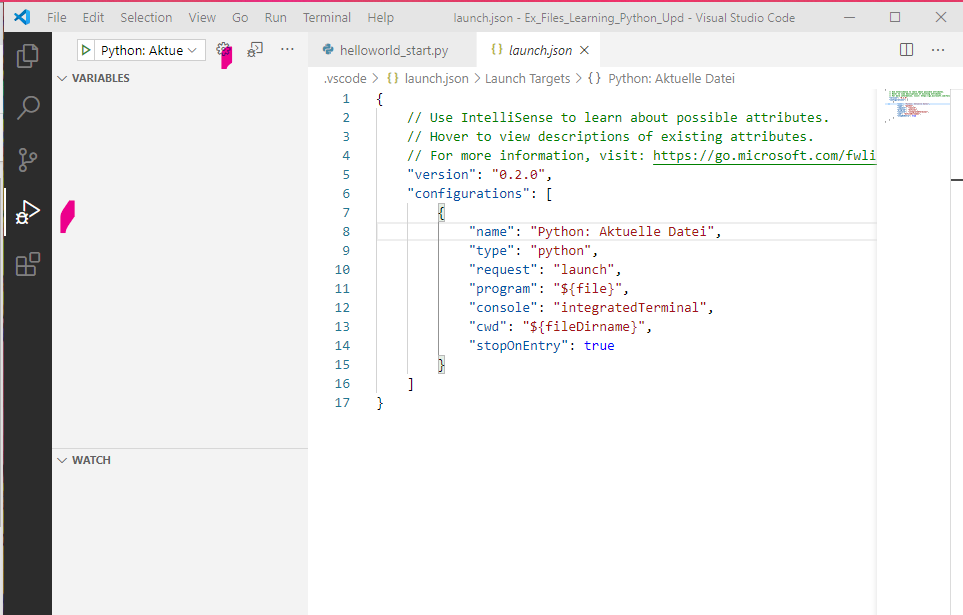
\includegraphics[scale = 0.3]{attachment/chapter_3/Scc069}
\caption{}
\label{fig:Scc069}
\end{figure}
\begin{itemize}
\item \bl{cwd} gibt an wo \textit{C}urrent\textit{W}orking\textit{D}irectory ist.
\item \bl{stopOnEntry} Stop den Vorgang zum Anfang der Datei
\end{itemize}

\subsubsection{Internal Console instead of Terminal}
Eine verschlankte Anzeige ist, wenn die Console nicht über das Terminal gestartet wird. Eine Einschränkung gibt es, Python kann keine Eingaben erhalten.
\begin{figure}[H]
\centering
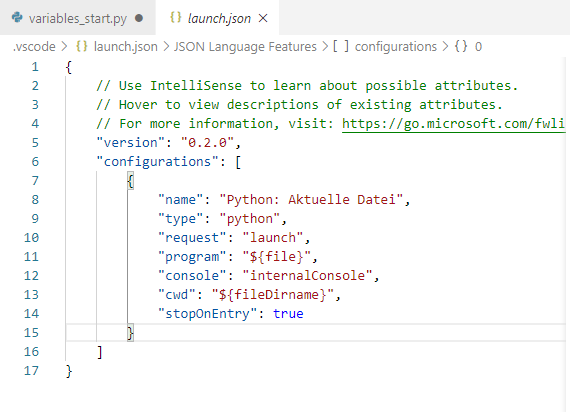
\includegraphics[scale = 0.2]{attachment/chapter_3/Scc070}
\end{figure}
\begin{itemize}
\item \bl{console} integratedTerminal - Vollumfang
\item \bl{console} internalConsole - Verschlankte Darstellung in Debug Console, Kein Input
\end{itemize}


\subsection{Basis Concepts}
\subsubsection{Variables and Expressions}
\begin{itemize}
\item Keine spezifische Typ Zuweisung
\item Die \bl{print()} Funktion muss gleiche Typen erhalten
\begin{lstlisting}[style=python]
	# Declare a variable and initialize it
	f = 0
	print(f)
	
	
	# re-declaring the variable works
	f = "abc"
	print(f)
	
	
	# ERROR: variables of different types cannot be combined
	'print("string" + 2)
	print("string"+str(2))
\end{lstlisting}
\item Innerhalb einer Funktion wird eine lokale Variable abgelegt.
\begin{lstlisting}[style=python]
	# Global vs. local variables in functions
	def someFunction():
	f = "def"
	print(f)
	
	someFunction()
	print(f)
\end{lstlisting}
Output:\\
def\\
f
\item Deklariert man die als \textit{global} wird die Variable außerhalb der Funktion ebenfalls neu definiert.
\begin{lstlisting}[style=python]
	\begin{lstlisting}[style=python]
		# Global vs. local variables in functions
		def someFunction():
		global f
		f = "def"
		print(f)
		
		someFunction()
		print(f)
	\end{lstlisting}
	Output:\\
	def\\
	def
	\item Eine Inputvariable mit einem * fungiert als Array.
\end{itemize}
\subsubsection{Function}
Funktion werden anders als in C++ nicht mit einem Funktionsrupf versehen. Ab wann die Rupf in pyhton anfängt wird mit $:$ und einer Einrückung versehen.

Die Print-Funktion ruft eine als Argument übergebenen Funktion auf und gibt den Wert der Funktion wieder. Damit ist der Return Wert gemeint, sondern der Allgemeine Wert einer Funtion - None.

Wenn die Funktion einen Return Wert besitzt, gibt Print() diesen wieder. Eine separate Ausgabe wird nicht durchgeführt.
\begin{lstlisting}[style=python]
	# function that returns a value
	def cube(x):
	return x*x*x
	
	print(cube(3))
	# 27
\end{lstlisting}
In \gls{g_Python} kann die Adressierung der Inputvariablen in einer Funktion getauscht werden.
\begin{lstlisting}[style=python]
	def func3(a,b):
	return a/b
	
	print(func3(3,2)) # 1.5
	print(func3(b=2, a=3)) 1.5
\end{lstlisting}

\subsubsection{Conditionals}
Der if-else Block unterscheidet sich zu C++ von der Syntax. Die Teilbereich des \bl{if} Blocks wird mit $:$ beendet. Ebenso gibt dies für \bl{else}.
Weil \gls{g_Python} eine Leerzeichen sensible Sprache ist, muss auf die Einrückung geachtet werden.

\begin{lstlisting}[style=python]
	def main():
	x, y = 1000, 100
	
	# conditional flow uses if, elif, else
	if x < y:
	str = "x is less than y"
	elif x==y:
	str = "x is equal to y"
	else:
	str = "x is greater then y"
	print(str)
	
	# conditional statements let you use "a if C else b"
	
	if __name__ == "__main__":
	main()
\end{lstlisting}
\subsubsection{Loop}
\begin{itemize}
	\item While Loop
	\begin{lstlisting}[style=python]
		# define a while loop
		while (x<5):
		print(x)
		if (x==3): break
		x = x + 1
	\end{lstlisting}
	Nach der Bedingung wird in \gls{g_Python} mit einem : beendet.
	\item For Loop
	\begin{lstlisting}[style=python]
		# define a for loop
		for x in range(5,10):
		print(x)
	\end{lstlisting}
	mit der Rang Funktion kann der Bereich definiert werden, welcher durchlaufen werden soll. Arrays können ohne Indexierung, wie in C++, durchlaufen werden.
	\begin{lstlisting}[style=python]
		# use a for loop over a collection
		days = ["Mo", "Di", "Mi", "Do", "Fr"]
		for d in days:
		if d == "Mi": break
		print (d)
	\end{lstlisting}
	oder 
	\begin{lstlisting}[style=python]
		# use a for loop over a collection
		days = ["Mo", "Di", "Mi", "Do", "Fr"]
		for d, i in enumerate(days):
		print (i, d)
	\end{lstlisting}
\end{itemize}

\subsection{OOP - Class}
\subsubsection{Structure of a Class}
Der einfachste Fall ist eine Klasse, die leer ist. Der Befehl nach der Definierung der Klasse ist \bl{pass}.\\

Ein Beispiel für eine Klasse mit zwei Methoden und einem belegten Attribute ist
\begin{lstlisting}[style=python]
	class myClass():
	# Attribute
	x = "Python"
	
	# Methode 1
	def Methode1(self):
	print("Output Methode 1 myClass")
	
	# Methode 2
	def Methode1(self, x):
	print("Output Methode 1 myClass" + x)
	
	object = myClass
	print(object.x) # Python
\end{lstlisting}
\subsubsection{Inheritance and Override}

Die Vererbung einer Klasse funktioniert von der Syntax ähnlich wie in \gls{CPP}. Die Superklasse oder Parentclass wird als Objekt in die Klasse übergeben.

\begin{lstlisting}[style=python]
	class ChildClassName(SuperClassName):
\end{lstlisting}
Die Methoden und Attribute der Superklasse werden vererbt. Mit Hilfe von Methode Override können die vererbten Methode geändert werden.\\

Im Folgenden wird die Superklasse \textbf{myClass()} an die Klasse \textbf{anotherClass()} übergeben.
\begin{lstlisting}[style=python]
	class myClass():
	def method1(self):
	print("myClass method1")
	
	def method2(self, someString):
	print("myClass method2: " + someString)
	
	def method3(self):
	print("myClass method 3")
	
	
	class anotherClass(myClass):
	def method1(self):
	print("anotherClass method1")
	
	def method2(self):
	print("anotherClass method2")
\end{lstlisting}
Hierbei werden \textit{method1} und \textit{method2} überschrieben. Die \textit{methode3} wird vererbt. 
Die Instanzierung beider Klassen erfolgt auf dem üblichen Weg
\begin{lstlisting}[style=python]
	instanzSK = myClass()
	instanzCK = anotherClass()
\end{lstlisting}
Die Methoden der Superklasse können über das erzeugt Objekt \textbf{InstanzSK} aufgerufen werden.
\begin{lstlisting}[style=python]
	instanzSK.methode1() # myClass method1
	instanzSK.methode2("Test") # myClass method2: Test
	instanzSK.methode3() # myClass method3
\end{lstlisting}
Die Instanz der Kindklasse hat die Möglichkeit die zwei überschriebenen Methode und die verrebte Methode aufzurufen.
\begin{lstlisting}[style=python]
	instanzCK.methode1() # anotherClass method1
	instanzCK.methode2() # anotherClass method2
	instanzCK.methode3() # myClass method3
\end{lstlisting}
Die Möglichkeit Methode Overload bei vererbten Methoden anzuwenden ist nicht möglich, siehe folgendes Beispiel:
\begin{lstlisting}[style=python]
	instanzCK.methode2("Test") # Error
\end{lstlisting}


\subsubsection{Methode Overload}
Das Prinzip von Methode Overload wird in \gls{g_Python} wird nicht wie in \gls{CPP} mit zwei gleichnamigen Funktionen mit unterschiedlicher Anzahl von Parametern umgesetzt. In \gls{g_Python} wird Methode Overload in einer Funktion vereinigt. Die Inputvariablen werden mit einem Default Wert besetzt. Wird dieser nicht übergeben, kann zwischen verschiedenen Bereichen in der Funktion unterschieden werden.\\

Würde die Logik von \gls{CPP} gelten, würde eine Ausführung wie folgt aussehen:
\begin{lstlisting}[style=python]
	class myClass():
	def method1(self):
	print("myClass method1")
	
	def method1(self, someString): # Zwei Parameter
	print("myClass method1: " + someString)	
	
	c = myClass()
	c.method1() # myClass methode1
	c.method1("Test") # myClass methode1: Test
\end{lstlisting}

Mit \gls{g_Python} wird dies in der Funktion mit einem Default Wert für \textit{someString} erreicht.
\begin{lstlisting}[style=python]
	class myClass():
	def method1(self, someString = None):
	if someString is None:
	print("myClass method1")
	else:
	print("myClass method1: " + someString)	
	
	c = myClass()
	c.method1() # myClass methode1
	c.method1("Test") # myClass methode1: Test
\end{lstlisting}

\subsubsection{The self Argument}
Klassen Methoden benötigen einen Parameter, welcher beim Aufrufen der Instanz nicht übermittelt werden muss. Dieser Parameter heißt \textit{self}. Er ist vergleichbar mit dem \textit{Me} Objekt im \gls{VBA}. In \gls{CPP} wird dies nicht benötigt. 
Die Instanz der Klasse übergibt den Wert von sich selbst an den \textit{self} Parameter. \\

Wird eine Klasse mit einer Methode erstellt:
\begin{lstlisting}[style=python]
	class myClass():
	def method1(self):
	print("myClass method1")
\end{lstlisting}
so kann diese über aufgerufen werden, indem eine Instanz der Klasse, \textit{c}, erstellt wird und die Methode direkt aufgerufen wird.
\begin{lstlisting}[style=python]
	c = myClass()
	c.method1() #
\end{lstlisting}
Der Wert des Objektes \textit{c} wird hierbei übergeben, ohne explizit genant zu werden.
Dies liegt an der Syntax. Voll ausgeschrieben wird die Methode \textit{method1()} über die Klasse selbst aufgerufen.
\begin{lstlisting}[style=python]
	myClass.methode1(c) # myClass method1
\end{lstlisting}

\subsubsection{Attributes}
Die Attribute eine Klasse können entweder einer Instanz oder der Klasse selbst zugeordnet werden.
Eine Variable deklarieren wird in \gls{g_Python} nicht in der Form getan, wie in \gls{CPP}.\\

\paragraph*{Ohne Constructur init ist falsch}
Um ein Attribute für jede Instanz ansteuerbar zu machen, muss das \textit{self} verwendet werden.
\begin{lstlisting}[style=python]
	class myClass():
	self.attribute # ERROR
	
	c = myClass()
	c.attribute = 5
	print(c.attribute)
\end{lstlisting}

\paragraph*{Mit Constructor init ist richtig}
Ein Attribut kann nur über die \textit{init} Methode deklariert werden.
\begin{lstlisting}[style=python]
	class myClass():
	def __init__(self,attribute)
	self.attribute = attribute		
	
	#c = myClass() # Error: Missing Input
	c = myClass(5)
	#c.attribute = 5 # Nicht mehr benötigt
	print(c.attribute) # 5
	c.attribute = 6
	print(c.attribute) # 6
\end{lstlisting}

\paragraph*{Attribut einer Klasse direkt zuordnen.}
Ein Attribut kann auch einer Klasse direkt zugeordnet werden. Dabei hat jede Instanz die Möglichkeit auf das Atrribute zuzugreifen und Änderungen vorzunehmen.
\begin{lstlisting}[style=python]
	class myClass():
	attribute1 = None
	def __init__(self,attribute2)
	self.attribute1 = attribute	
	
	c = myClass(5)
	cc = myClass(6)
	myClass.attribute1 = 3
	
	# Check Attribute1
	print(c.attribute1) # 3
	print(cc.attribute1) # 3
	print(myClass.attribute1) # 3 
	
	# Check Attribut2
	print(c.attribute2) # 5
	print(cc.attribute2) # 6
\end{lstlisting}

Es ist Achtsamkeit geboten, wenn eine Klassen Attribute von einer Instanz geändert wird, wird dieser Instanz das Attribut als eigenständige Variable zugeordnet.

\begin{lstlisting}[style=python]
	class myClass():
	attribute1 = None
	def __init__(self,attribute2)
	self.attribute1 = attribute	
	
	c = myClass(5)
	cc = myClass(6)
	
	
	# Change Class Attribute over class itself
	myClass.attribute1 = 3
	print(c.attribute1) # 3
	print(cc.attribute1) # 3
	print(myClass.attribute1) # 3
	
	# Class attribute changes to instanz attribute
	c.attribute1 = 9
	print(myClass.attribute1) # 3
	print(c.attribute1) # 9
	print(cc.attribute1) # 3
	
	# New instanz varialbe stays the same
	myClass.attribute1 = 10
	print(myClass.attribute1) # 10
	print(c.attribute1) # 9
	print(cc.attribute1) # 10
\end{lstlisting}

\subsubsection{Call methode from another Class}
Jede Methode einer Klasse ist ebenfalls von Instanzen andere Klassen nutzbar. Die zu übergebenen Parameter müssen von der Fremde-Instanz auch bereit gestellt werden. Es müssen nicht alles Eigenschaften Fremden-Instanz gleich sein, nur die, die für die aufgerufenen Methode benötigt wird.\\

Der Parameter \textit{\bl{self}} bezieht sich auf die Fremde-Instanz.
\begin{lstlisting}[style=python]
	class myClass():
	def __init__(self, a, b):
	self.a = a
	self.b = b
	def method1(self):
	print("Method1 myClass: ", self.a, self.b)
	self.a = self.a + 1
	print("Method1 myClass: ", self.a, self.b)
	
	class anotherClass():
	def __init__(self, a, b):
	self.a = a
	self.b = b
	def method1(self):
	A = myClass(2,2)
	print("Method1 anotherClass")
	myClass.method1(A) # equal to self.method1()
	
	class tanotherClass():
	def __init__(self, a, b):
	self.a = a
	self.b = b
	
	def method1(self):
	print("Method1 tanotherClass")
	myClass.method1(self)
	
	c  = myClass(1,1)
	cc = anotherClass(4,4)
	ccc= tanotherClass(8,8)
	
	c.method1() 	# Method1 myClass: " 1 1
	# Method1 myClass: " 2 1
	cc.method1() 	# Method1 anotherClass
	# Method1 myClass: " 2 2
	# Method1 myClass: " 3 3
	
	cc.method1() 	# Method1 tanotherClass
	# Method1 myClass: " 8 8
	# Method1 myClass: " 9 8
	
	
\end{lstlisting} 
Wird die Klasse \textit{myClass} als Superklasse übergeben, benötigt es \textit{init} nicht mehr.
\begin{lstlisting}[style=python]
	class anotherClass(myClass): # Vererbung von __int__
	def method1(self):
	A = myClass(2,2)
	print("Method1 anotherClass")
	myClass.method1(A) # equal to self.method1()
\end{lstlisting}


\subsubsection{Public, Private and Protected}
\begin{description}
	\item[Protected] Eine Variable kann als privat deklariert werden. Es gibt aber von \gls{g_Python} kein Einschränkungen. Syntax $\_$. Die Konvention ist, dass der Zugang zu den geschützten Attribute (Variablen) nur über get und set Funktionen erfolgt.
	\begin{lstlisting}[style=python]
		class myClass():
		def __init__(self, a, b):
		self._a = a
		self.b = b
		
		c = myClass(5,6)
		print(c._a, c.b) # 5 6
	\end{lstlisting}
	\item[Private] Eine Variable kann als privat deklariert werden. Eine direkte Aufrufen
	\begin{lstlisting}[style=python]
		c = myClass(5,6)
		print(c.__b) # Error, wenn self.__b = b
	\end{lstlisting} Über eine andere Syntaxt ist dies aber möglich.
	\begin{lstlisting}[style=python]
		class myClass():
		def __init__(self, a, b):
		self._a = a
		self.__b = b
		
		c = myClass(5,6)
		print(c._a, c._myClass__b)
	\end{lstlisting}
\end{description}

\subsubsection{From ... import}
Der erste Teil \textit{From ...} verweist auf das komplette Modul. Der zweite Teil referiert auf eine spezifische Klasse.

\subsection{Modul Formating Date and Time}
\begin{itemize}
	\item Das Packet \textit{datetime} besteht aus mehrern Klassen. Eine davon lautet ebenso \textit{datetime}. 
	\item Information zu dem Module findet sich unter \href{https://docs.python.org/3/library/datetime.html}{Python Library}
\end{itemize}

\subsubsection{Retriev information form datetime module with date, time and datetime class}
\begin{lstlisting}[style=python]
	from datetime import date
	from datetime import time
	from datetime import datetime
	
	def main():
	## DATE OBJECTS
	# Get today's date from the simple today() method from the date class
	today = date.today()
	todaytime = datetime.today()
	
	# print out the date's individual components
	print("Day:", today.day) # equal to date.today().day
	print("Month:", today.month) 
	print("Year:", today.year)
	
	print("Datetime: ", datetime.today())
	print(datetime.today().day) # equal to todaytime.day
	print(datetime.today().month)
	print(datetime.today().year)
	print(datetime.today().hour)
	
	
	# retrieve today's weekday (0=Monday, 6=Sunday)
	print("Weekday:", today.weekday())
	print("Weekday:", date.today().weekday())
	
	weekdays = ["Mo", "Di", "Mi", "Do", "Fr", "Sa", "So"]
	print("Weekday full name: ", weekdays[date.today().weekday()])
	
	## DATETIME OBJECTS
	# Get today's date from the datetime class
	print("Date form Datetime class:", datetime.date(datetime.today())) # .date() benötigt eine Input
	
	# Get the current time
	print("Current Time:", datetime.time(datetime.today()))
\end{lstlisting}

\subsubsection{Formating}
Die Funktion \textit{str()} wandelt eine Input Objekt in einen String um. 
\begin{lstlisting}[style=python]
	str(5) # converts a integer to a string
	int("5") # converts a string to an integer
\end{lstlisting}

Die Funktion \textit{strftime()} bekommt vom vererbten Objekt den datetime oder date Input. Die Methode funktioniert, in der Hinsicht, dass die Methode formattierte Strings ausgeben kann. Dabei können auch mehrere Formatierungscodes angegeben werden: 
\begin{itemize}
	\item * Alle Codierungen werden mit einem führenden Prozentzeichen angegeben.
	\item m - Monat, b - Monatsname Kurz, B - Monatsname Lang
	\item d - Tag, w - weekdat
	\item y - Jahr
	\item H - Stunde, I - Stunden (12-Stunden Uhr) mit einer führenden Null, -I - Stunden (12 Uhr) als Dezimazahl, p - Local AM or PM
	\item M - Minute
	\item S- Sekunde
\end{itemize}
\begin{lstlisting}[style=python]
	#
	# Example file for formatting time and date output
	#
	
	from datetime import datetime
	
	def main():
	# Times and dates can be formatted using a set of predefined string
	# control codes 
	print("Now", datetime.now()) 
	print("Now", datetime.now().today()) # returns the same as before and after this linie
	print("Today", datetime.today()) # returns the same output as now()
	
	#### Date Formatting ####
	
	### strftime() datetime, date to string
	# %Y, %m, %d, %y/%Y - Year, %a/%A - weekday, %b/%B - month, %d - day of month are Format Codes.
	print(datetime.today().strftime("%Y")) # 2020
	print(datetime.now().strftime("%H:%M:%S"))  # 20:49:31
	
	
	# %c - locale's date and time, %x - locale's date, %X - locale's time
	print(datetime.today().strftime("%c")) # Full Formation
	print(datetime.today().strftime("%x"))
	print(datetime.today().strftime("%X"))
	if __name__ == "__main__":
	main()
\end{lstlisting}
Der umgedrehte Fall folgt aus \textit{strptime()}. Die Methode nimmt einen String und wandelt in ein datetime Objekt um.
\subsubsection{Timedelta}
Mit \textit{timedelta()} kann eine Zu- oder Abbuchung auf ein date oder datetime Objekt erfolgen.
\begin{lstlisting}[style=python]
	from datetime import datetime
	from datetime import date
	from datetime import time
	from datetime import timedelta
	
	print("One year form now:", date.today() + timedelta(days=365)) # 08.12.2021
	print("One year form now:", datetime.now() + timedelta(days=365)) # 08.12.2021 10:11:223
\end{lstlisting}
Die Funktion \textit{retrieve()} ermöglicht es bestimmte Bestandteilen einer \textit{datetime()} und oder \textit{date()} Variable zu ändern.

\begin{lstlisting}[style=python]
	### How many days until April Fools' Day?
	xmas = date(2020,12,24)
	
	if date.today() == xmas:
	print("Today ist Christmas.")
	xmas = xmas + timedelta(weeks=52)
	print("Nächstes Weihnnachten ist ", xmas)
	else:
	print("Es sind noch", (date.today() - xmas).days, "Tage")
	
	# use date comparison to see if April Fool's has already gone for this year
	# if it has, use the replace() function to get the date for next year
	print("Alternativ kann das Datum mit replace() ermöglicht werden.", xmas.replace(year=date.today().year +2))
\end{lstlisting}

Eine Subtraktion von zwei Daten wird als ein Objekt umgewandelt, welches die Tage zwischen den zwei Daten zählt.
\begin{lstlisting}[style=python]
	d = date.today()
	b = date(2019,6,15)
	print(d-b) # Returns 549 days, 0:00:00
	print(d+b) # Returns Error
\end{lstlisting}
Die Operation $-$ ist für \textit{datetime.date} Objekte definiert. Die Addition nicht.
Die Operation Subtraktion wandelt $d-b$ in ein Objekt \textit{datetime.timedelta} um. Es handelt sich hierbei nicht um ein Integer.
Um einen Vergleich mit zwei Zahlen zu ermögliche, muss ein Tag, Jahr oder Monat aus dem \textit{Timedelta} Objekt extrahiert werden.
\begin{lstlisting}[style=python]
	d = date.today()
	b = date(d.year,6,30)
	diff = (d-b).days # OHNE Days kommt es zu einen Instanzen-Fehler
	if diff > 0:
	print("Birthday in %d days" % diff)
	else:
	print("Birthday in %d days" % diff)
\end{lstlisting}

\subsubsection{Calendar}
Unter \href{https://docs.python.org/3/library/calendar.html}{Library Calendar} wird der Aufbau des Moduls \textit{calendar}.

Die Aufbau sieht wie folgt aus:
\begin{itemize}
	\item Über das Modul selbst können einfache Kalender erstellt werden.
	\begin{lstlisting}[style=python]
		c = calendar
	\end{lstlisting}
	\item Das Objekt \textit{c} besitzt Methoden und Attribute. Die Klasse dient zur Vorbereitung von Kalendar Informationen. Eine Formatierung ist nicht über die Klasse vorgesehen.
	\begin{lstlisting}[style=python]
		import calendar
		c = calendar.calendar
	\end{lstlisting}
	\item Detailtiere Kalender können über 
	\begin{lstlisting}[style=python]
		import calendar
		c = calendar.TextCalendar(firstweekdays=) # oder
		c2 = calendar.HTMLCalendar(fristweekdays=)
	\end{lstlisting}
	erstellt werden.
\end{itemize}

\paragraph*{Beispiele}

\begin{itemize}
	\item calendar.weekday(year, month, day) Returns the day of the week.
	\item calendar.weekheader(n) Returns header abbreviated
	\item calendar.monthcalendar(year,month) Returns a matrix representing a tupels of days. Example .monathcalendar(2020,2) 
	\begin{align}
		\rightarrow \left[\left[0, 0, 0, 0, 0, 1, 2\right], \left[3, 4, 5, 6, 7, 8, 9\right], \left[10, 11, 12, 13, 14, 15, 16\right],\right. \\
		\left.\left[17, 18, 19, 20, 21, 22, 23\right], \left[24, 25, 26, 27, 28, 29, 0\right]\right]
	\end{align}
	\item calendar.MONDAY gibt den Integer 0 wieder. Von Montag bis Sonntag ist dies möglich mit 0-6
	\item calendar.week(theweek, w) gibt einen cal Kalender mit Titel und Wochen Bezeichnung wieder.
	\item calendar.TextCalendar(calendar.SUNDAY) gibt ein HTML Objekt wieder, welches weiter formatiert und dargestellt wird.
	\item calendar.TextCalendar(calendar.SUNDAY).formatyear(theyear=2020, w=4) gibt einen komplette Kalender des Jahres 2020 wieder.
	\item calendar.TextCalendar(calendar.SUNDAY).formatmonat(theyear=2020, themonth=12, w=4) gibt einen kompletten Monatskalender wieder.
	\item calendar.TextCalendar(calendar.SUNDAY).formatweek(theweek=[(0,6),$\dots$], w=4) gibt eine Liste von Datumstagen wieder.
\end{itemize}



\subsection{Working with files}
Python bietet einen Sammelsurium von Build-In Funktionen an, siehe \href{https://docs.python.org/3/library/functions.html}{Python Libary.}
\begin{figure}[H]
	\centering
	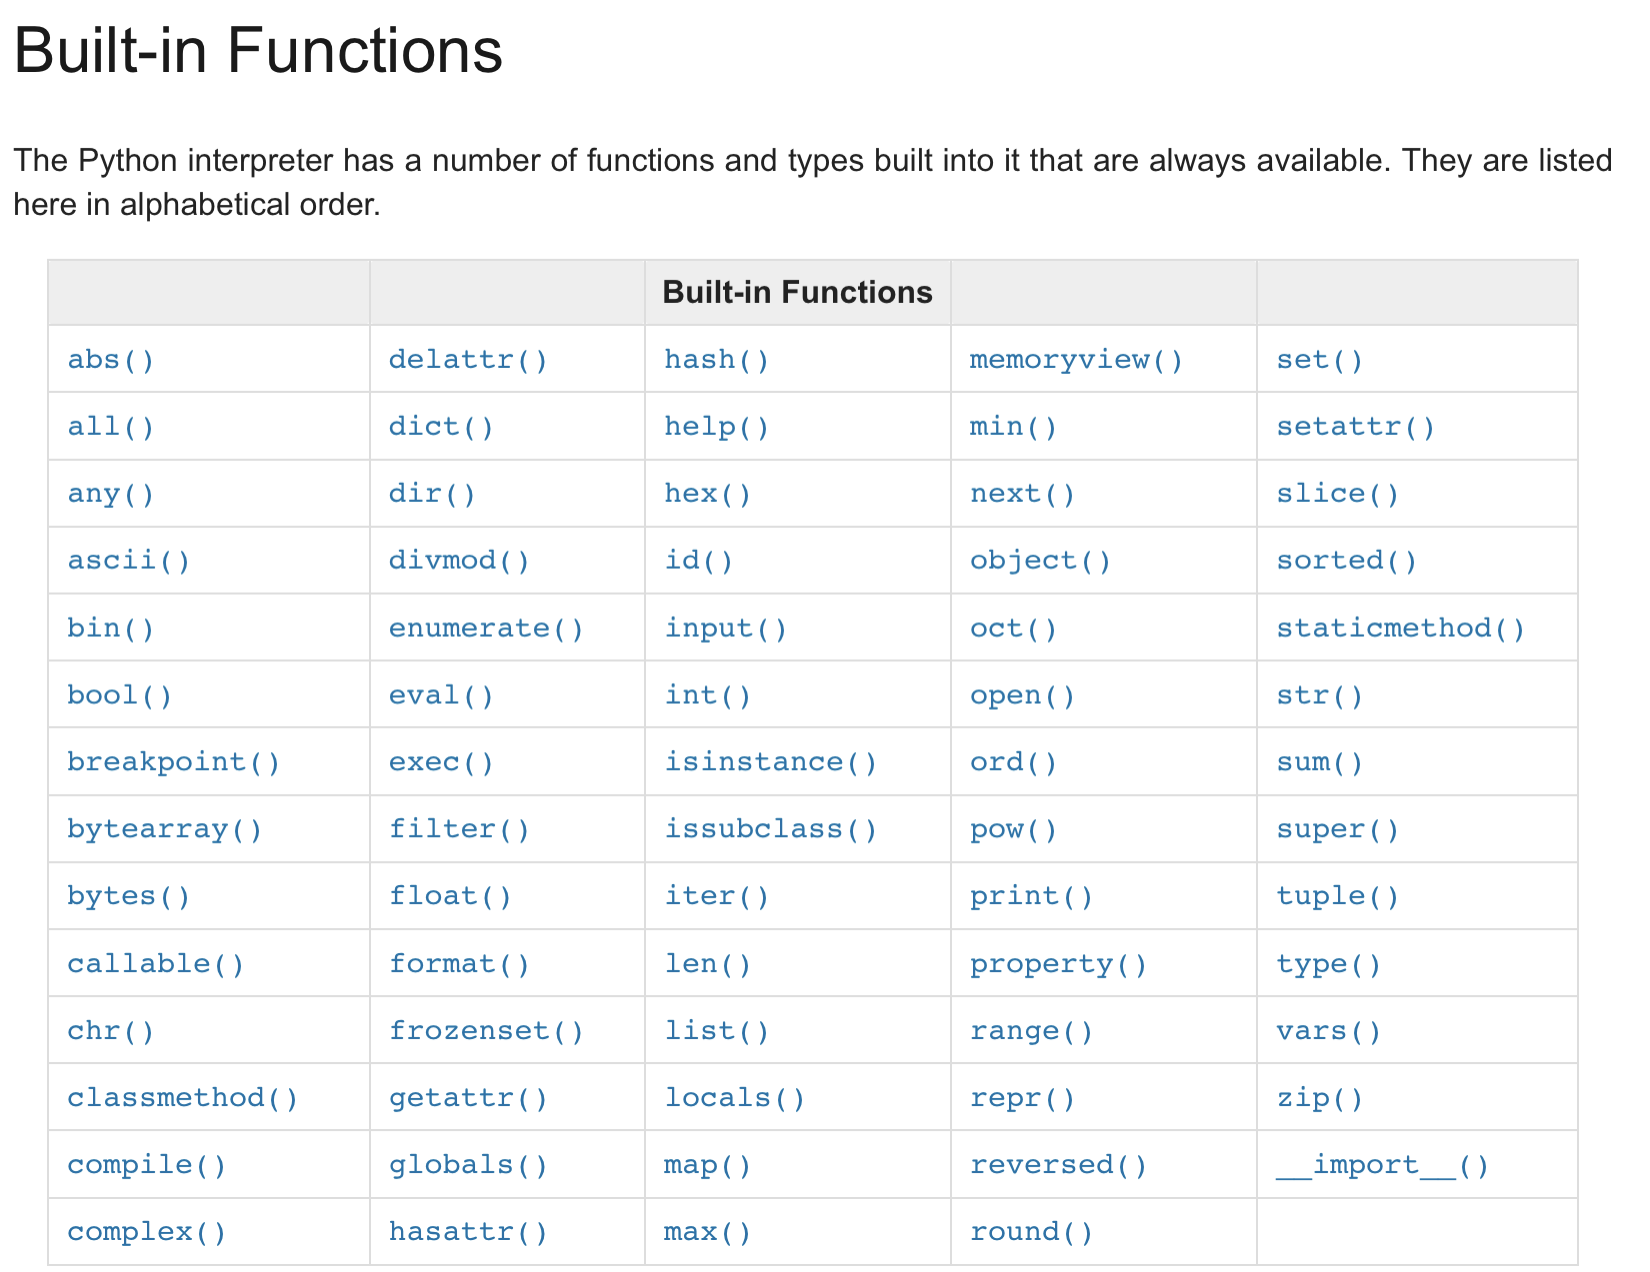
\includegraphics[scale = 0.3]{attachment/chapter_3/Scc071}
\end{figure}

\subsubsection{Open(File,Mode)}
Eine Funktion \textit{open()} gibt einen Zugang zu Dateien, um diese zu ändern und anzupassen. Die wichtigesten Parameter, welche die Datei aufnimmt, sind 
\begin{itemize} 
	\item file - gibt an, wo die Datei zu finden ist und den Namen der Datei. Wir kein direkter Pfad angegeben, muss die Datei im gleichen Verzeichnis liegen, wo auch die .py liegt.
	\item modus - gibt an, in welchem Modus die Datei verwendet werden soll.
	\begin{itemize}
		\item $"$r$"$ - Read
		\item $"$w$"$ - Write and Trunciation (Kürzen: Datei wird geleert.)
		\item $"$a$"$ - Append
		\item $"$r+$"$ - Read and Write
		\item $"$x$"$ - Creating (Error, if file exist)
	\end{itemize}
\end{itemize}
Die Funktion erzeugt ein File-Objekt. Die einfachste Objekt-Methode ist \textit{.close()}.
\begin{lstlisting}[style=python]
	# open(file,modus)
	fileObject = open("Testfile.txt","r")
	fileObject.close() # Some Changes are only taking effect after the file is closed. 
\end{lstlisting}
Dies ist wichtig, um Überschreibungen, Fehler und Ladungen richtig durchzuführen.

Das Objekt, je nach Modus, besitzt mehrere Attribute und Methoden.
\begin{lstlisting}[style=python]
	# open(file,modus)
	file = open("Testfile.txt","r")
	print(file.name) # Testfile.txt
	file.close() 
\end{lstlisting}

Die Ausgabe der Datei funktioniert über \textit{.read().} Der Modus \textit{r} muss aktivert sein, damit eine Ausgabe möglich ist. Der Modus \textit{w} erlaubt die Methode nicht.
\begin{lstlisting}[style=python]
	# open(file,modus)
	file = open("Testfile.txt","r")
	print(file.read()) # Ausgabe des Inhaltes der Datei
	file.close() 
\end{lstlisting}
Nach dem die Methode durchgeführt wird, befindet sich der Pointer (Cursor) am Ende der Datei ein mehrmaliges Auslesen ist damit nicht möglich. Um genauer zu sein, die Ausgabe bleibt leer. Um den Pointer wieder auf den Start der Datei zu legen, wird \textit{.seek()} benötigt.
\begin{lstlisting}[style=python]
	# open(file,modus)
	file = open("Testfile.txt","r")
	print(file.read()) # Ausgabe des Inhaltes der Datei
	file.seek(0) # setzt den Point auf den Anfang der Datei.
	print(file.read()) # Die Ausgabe kann komplett durchgeführt werden.
	file.close() 
\end{lstlisting}
Um spezifische Zeilen anzusteuern oder mehrmaliges Auslesen zu ermögliche, wird \textit{.readline()} oder \textit{.readlines()}. 

Die nächste Aufgabe befasst sich damit mehrer Zeilen in die Datei zu schreiben.
\begin{lstlisting}[style=python]
	file = open("test.txt","r+")
	for i in range(3,10):
	file.write("Das ist brilliant hoch " + str(i) + \n \r) 	file.close()	
\end{lstlisting}

Überträgt man die Daten der Auslesung, können die Daten in einer separaten Variable gespeichert werden.
\begin{lstlisting}[style=python]
	file = open("test.txt","r")
	if file.mode == "r": # Überprüft, ob die Datei richtig geöffnet wurde
	fileArray = file.readlines()
	for x in fileArray:
	print(x)
	
	file.close()	
\end{lstlisting}
Jede Zeile wird als Eintrag in dem Array abgespeichert, und kann auch als solches abgerufen werden.

\subsubsection{OS and OS.Path}

Das Paket OS erlaubt Zugriff auf das Datensystem. Path hat Funktionen implementiert, welche Operationen auf den Pfad und verbundenen Attribute erlaubt.

\begin{lstlisting}[style=python]
	from os import path
	
	# Check for item existence and type
	var1 = path.exists("textfile.txt")
	var2 = path.isfile("textfile.txt")
	var3 = path.isdir("textfile.txt")
	
	# Work with file paths
	var1 = path.realpath("textfile.txt")
	var2 = path.split(path.realpath("textfile.txt"))
	
	# Get the modification time
	var3 = path.getmtime("textfile.txt")
	var4 = path.getatime(path.realpath("textfile.txt")) # Der Path ist gleich gesetzt mit denm 
\end{lstlisting}

\subsubsection{Shutil and Zip}
Mit dem vorherigen Modul path konnten Dateinamen und Dateiverzeichnisse bearbeitet werden. Um Dateien zu bearbeiten, kopieren, verschieben und Operationen an mehrere Dateien durchzuführen, hilft \textit{Shutil}. Dateien können kopiert werdern.

Im Folgenden wird eine Kopie von der Beispieldatei textfile.txt erstellt und ein Archive des Ordners als Zip erstellt. Hinweis: Die Funktion .realpath() wirkt nur auf das aktuelle Verzeichnis. 

\begin{lstlisting}[style=python]
	#
	# Example file for working with filesystem shell methods
	#
	import os
	from os import path
	import shutil
	
	def main():
	# make a duplicate of an existing file
	if path.exists("textfile.txt"):
	# get the path to the file in the current directory
	sorginal = path.realpath("textfile.txt")
	scr = path.split(sorginal)
	scrG = str(scr[0])+str("/") + str(scr[1])
	dcr = scr[0] + str("/") + str("textfile-Copy.txt")
	# let's make a backup copy by appending "bak" to the name
	
	shutil.copy(sorginal, dcr)
\end{lstlisting}

Die Funktion \textit{.copystat()} transferiert Metadaten einer Datei zu einer anderen. 
\begin{lstlisting}[style=python]
	shutil.copy(sorginal, dcr)
	shutil.copystat(sorginal, dcr) # Transfer Metadaten
\end{lstlisting}

Um eine den Namen zu ändern, wird das Paket \textit{OS} verwendet. Mit \textit{.rename(scr,dcr)} wird das Attribute umgeschrieben.
\begin{lstlisting}[style=python]
	os.rename(sorginal, "textNew.txt")
\end{lstlisting}

Shutil enthält \textit{make}$\_$\textit{archive}. Zip-Dateien können somit gebildet werden.
\begin{figure}[H]
	\centering
	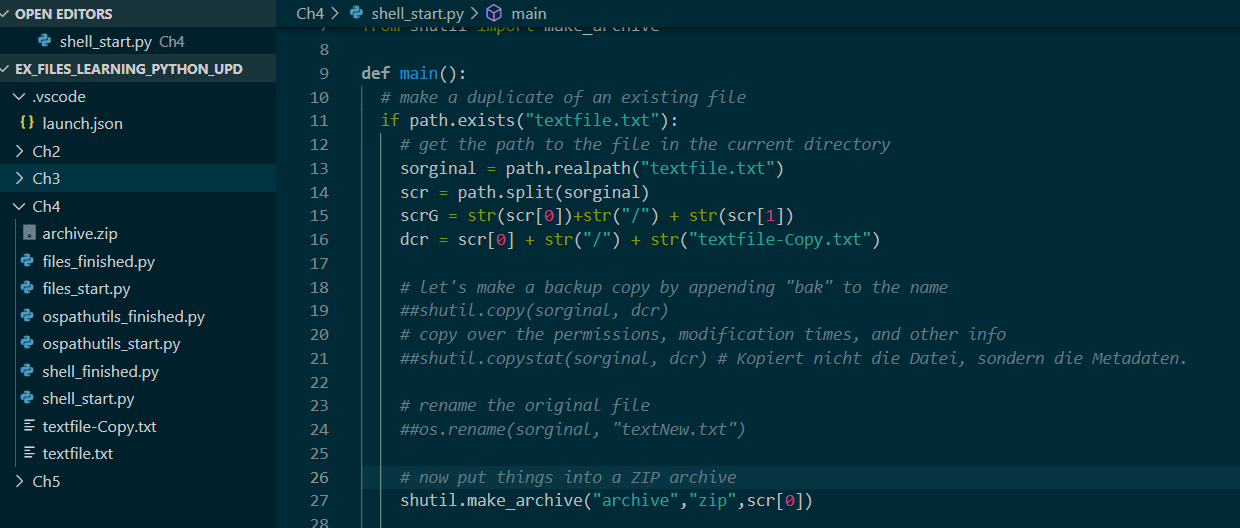
\includegraphics[scale = 0.3]{attachment/chapter_3/Scc072}
\end{figure}

Speziell für Zip Archive gibt es das Modul \textit{zipfile}. Aus dem Modul wird im folgenden Beispiel das Objekt \textit{ZipFile} importiert. Dies erlaubt eine genauere Bestimmung, was in das Archive hinein soll und was nicht.
\begin{lstlisting}[style=python]
	from zipfile import ZipFile
	# more fine-grained control over ZIP files
	with  ZipFile("testZip.zip","w") as newzip:
	newzip.write(path.realpath("files_start.py"))
	newzip.write(sorginal)
\end{lstlisting}

\subsection{Working with Webdata} 
\subsubsection{Urllib Request}
Das Paket \textit{urllib} enthält mehre Module
\begin{itemize}
	\item urllib.request
	\item urllib.error
	\item urllib.parse
	\item urllib.robotparser
\end{itemize}
das Modul \textit{urllib.request} hat die Funktion \gls{URL}s in \gls{HTTP} abzurufen. Mit \textit{.getcode()} wird eine Zahl wiedergeben, welche Auskunft über den Status des Abrufen der \gls{URL} gibt.
Es gibt folgende Klassen, welche angeben, ob eine Anfrage erfolgreich war:
\begin{itemize}
	\item Informational responses (100–199)
	\item Successful responses (200–299)
	\item Redirects (300–399)
	\item Client errors (400–499)
	\item Server errors (500–599)
\end{itemize}

Am Beispiel der \href{http://www.google.com}{Google-Startseite}, ist die Abfrage erfolgreich.
\begin{lstlisting}[style=python]
	webUrl = urllib.request.urlopen("http://www.google.com")
	print(str(webUrl.getcode())) # Returns 200 (if the request was successfull)
\end{lstlisting}

Mit \textit{.read()} wird die komplette \gls{HTTP}-Seite ausgelesen. Die Daten werden in dem Beispiel der Variable \textit{data} übergeben.
\begin{lstlisting}[style=python]
	data = webUrl.read()
	print(data)
\end{lstlisting}
Achtung: Selbst bei einfachen Seiten ist die Menge der ausgelesenen Daten hoch. Eine Darstellung über die Konsole kann daher eine hohe Rechenzeit benötigen.

\subsubsection{JSON}
Im diesem Beispiel soll es darum gehen, wie Daten aus dem Web per \gls{J.json} Format ausgelesen werden können. 
Die Daten beziehen sich auf die Seismischen Erdbeben Daten.
\begin{figure}[H]
	\centering
	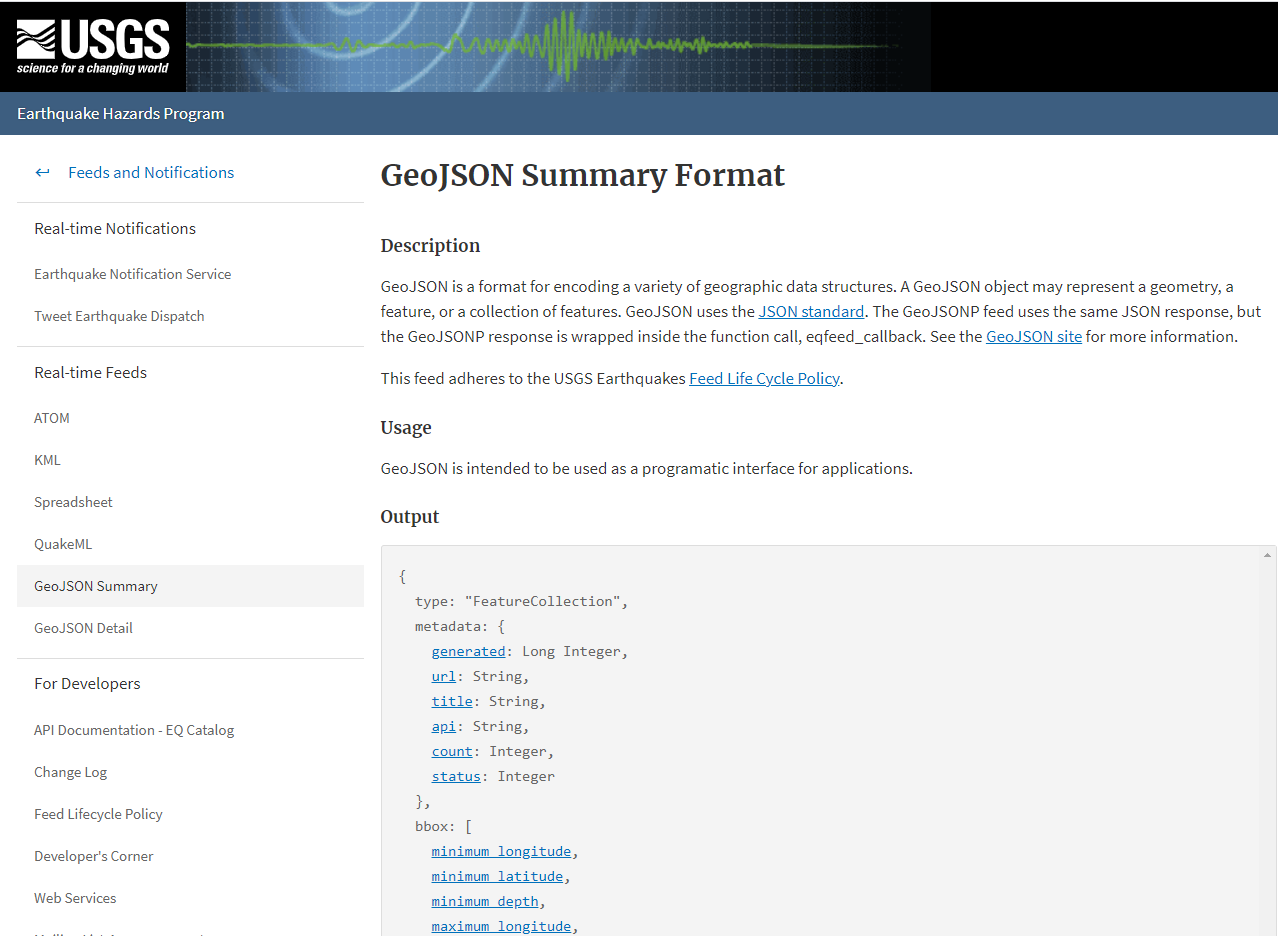
\includegraphics[scale = 0.3]{attachment/chapter_3/Scc073}
\end{figure}
Der Aufbau der Daten findet sich teilweise wie folgt aus:
\begin{figure}[H]
	\centering
	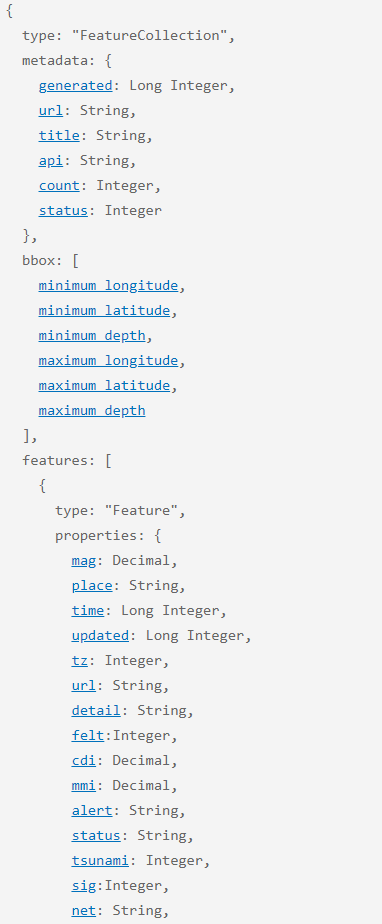
\includegraphics[scale = 0.3]{attachment/chapter_3/Scc074}
\end{figure}

Im ersten Schritt wird das Objekt erzeugt, welches die \gls{URL} öffnet: \textit{.request.urlopen()}. Um zuprüfen, ob die Webseite sich anfragen lässt, wird der \gls{HTTP} Code abgefragt. Ist dies Kontrolle positiv, wird die Webseite, die die \gls{J.json} Datei enthält, ausgelesen: \textit{.request.urlopen().read()}. Die Daten werden der Funktion \textit{printResults} übergeben.
\begin{lstlisting}{style=python}
	def main():
	# define a variable to hold the source URL
	# In this case we'll use the free data feed from the USGS
	# This feed lists all earthquakes for the last day larger than Mag 2.5
	urlData = "http://earthquake.usgs.gov/earthquakes/feed/v1.0/summary/2.5_day.geojson"
	
	# Open the URL and read the data
	webUrl = urllib.request.urlopen(urlData)
	if webUrl.getcode() == 200:
	printResults(webUrl.read())
	else:
	print("Seite lässt sich nicht öffnen.")
\end{lstlisting}

Mit dem Paket \textit{JSON} welches \gls{J.json} Formate entschlüsselt oder Daten in solche umwandelt.
\begin{itemize}
	\item String ($""$)
	\item Boolom (false, true)
	\item Integer (10, 1.5, -4, $\dots$)
	\item null 
	\item Array ($\left[...\right]$)
	\item Object ($\left\lbrace \dots \right\rbrace$)
\end{itemize}  Die Funktion \textit{.loads()} ließt die Erdbebendaten ein. Diese können jetzt wie im Beispiel direkt angesteuert werden. Im Glossar wird auf die Logik von \gls{J.json} eingegangen.
\begin{lstlisting}[style=python]
	
	def printResults(data):
	# Use the json module to load the string data into a dictionary
	theJSON = json.loads(data)
	
	# now we can access the contents of the JSON like any other Python object
	if "title" in theJSON["metadata"]:
	print(theJSON["metadata"]["title"])
	print(theJSON["metadata"]["api"])
	
	# All bbox entries
	for x in theJSON["features"]:
	print("Eigene Objekte:" + str(x) +"\n")
\end{lstlisting}

\begin{figure}[H]
	\centering
	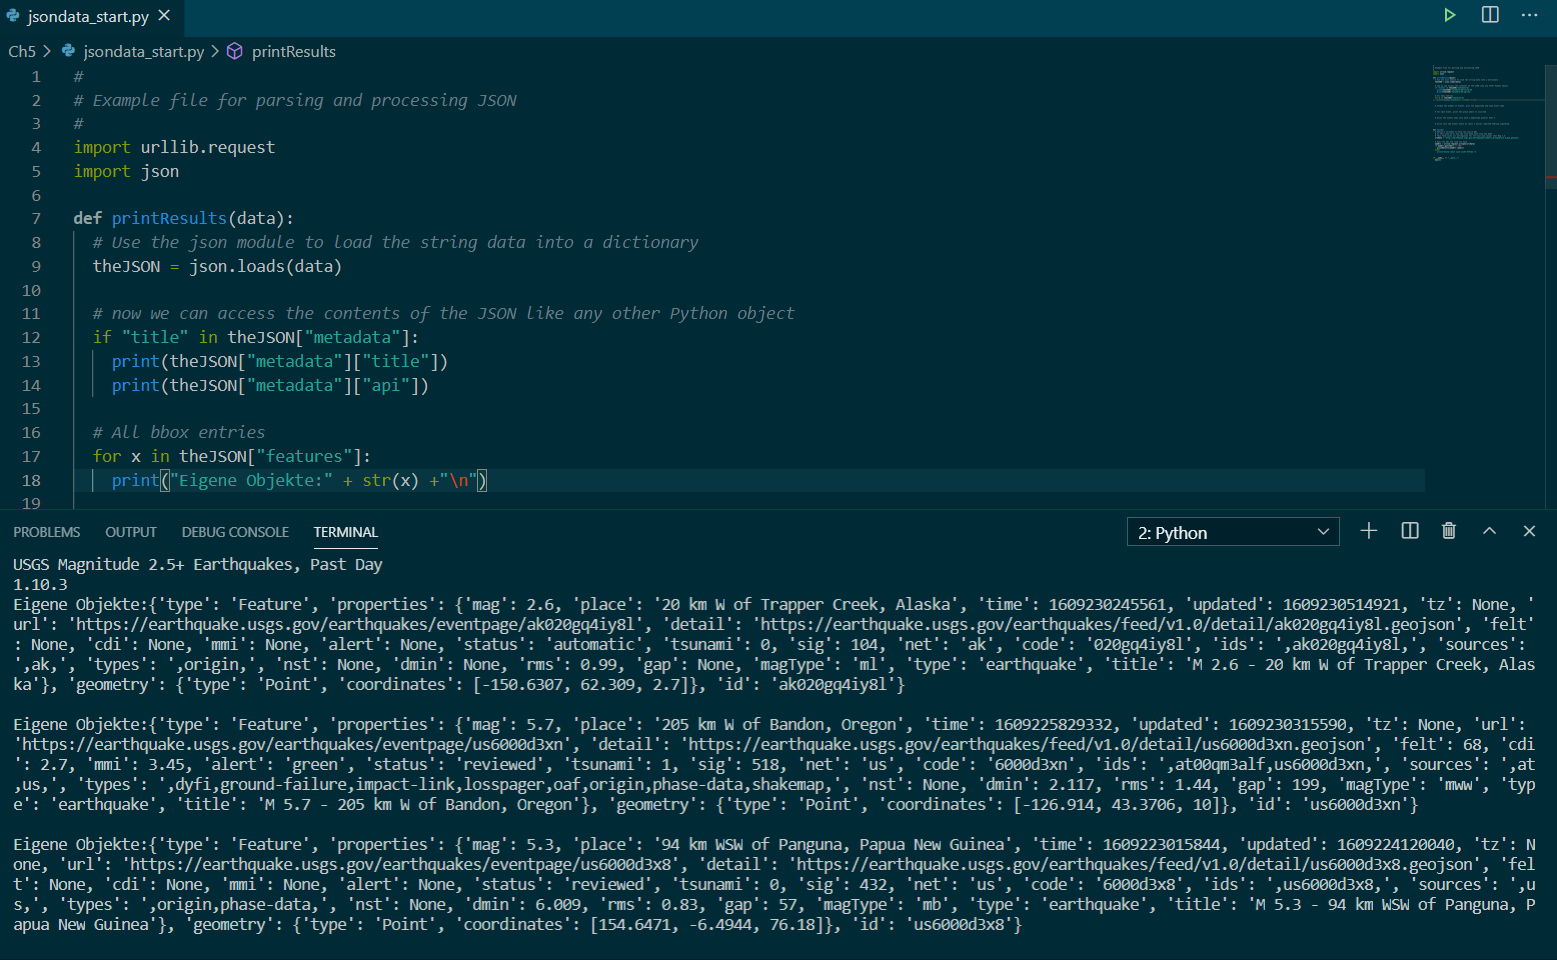
\includegraphics[scale = 0.3]{attachment/chapter_3/Scc075}
	\caption{Ausgabe: JSON}
\end{figure}  

Weite Aufgaben wurden gestellt, um spezifische Anfragen an die Erdbebendaten zu stellen.
\begin{lstlisting}[style=python]
	def printResults(data):
	# Use the json module to load the string data into a dictionary
	theJSON = json.loads(data)
	
	# now we can access the contents of the JSON like any other Python object
	if "title" in theJSON["metadata"]:
	print(theJSON["metadata"]["title"])
	print(theJSON["metadata"]["api"])
	print(theJSON["metadata"]["count"])
	
	# All bbox entries
	y = 0
	for x in theJSON["features"]:
	y += 1
	print("Eigene Objekte:" + str(x) +"\n")
	
	
	# output the number of events, plus the magnitude and each event name  
	print(str(y))
	
	# for each event, print the place where it occurred
	for x in theJSON["features"]:
	print("Ort: "+ str(x["properties"]["place"]) + " mit " + str(x["properties"]["mag"]))
	
	# print the events that only have a magnitude greater than 4
	for x in theJSON["features"]:
	if x["properties"]["mag"] >=4:
	print(x["properties"]["place"])
\end{lstlisting}

\subsubsection{HTML Parser (Plus: itertools)}
Mit dem Modul \textit{html.parser} ist eins von 4 Submodul von \gls{HTML}:
\begin{itemize}
	\item \textit{html.escape} converts special \gls{HTML} in strings.
	\item \textit{html.unescape} converts named and numeric character references in stings.
	\item \textit{html.entities} definies dictionaries.
\end{itemize} 

Mit \textit{parser} wird einen \gls{HTML} String durchsucht - dies kann zu einer Datei oder direkt zu einer Webseite referieren.
Das Modul besitzt nur eine Klasse - \textit{HTMLparser}. Anders, als bei anderen Modulen, wird hier eine abgeleitete (Sub-Klasse) Klasse gebildet.
\begin{figure}[H]
	\centering
	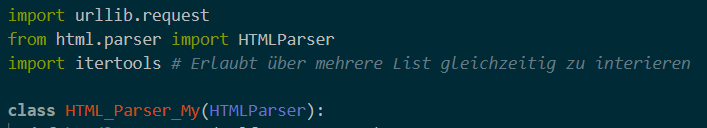
\includegraphics[scale = 0.3]{attachment/chapter_3/Scc076}
\end{figure} 
Der Input \textit{HTMLParser} dient als Referenzpunkt zur Hauptklasse. Die Klasse, \textit{HTMLParser} bietet Methoden an, welche überschrieben werden können. Diese nennen sich \textit{handler}
\begin{figure}[H]
	\centering
	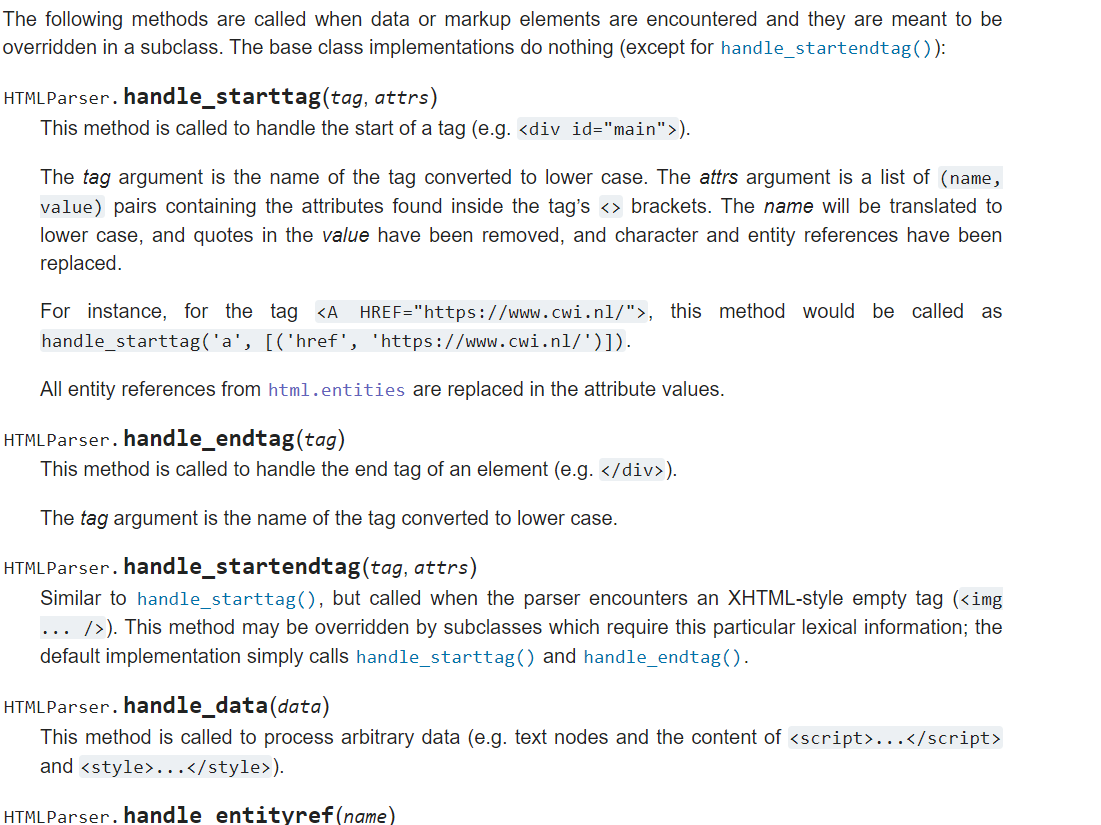
\includegraphics[scale = 0.3]{attachment/chapter_3/Scc077}
\end{figure} 
Beim Einlesen des \gls{HTML}-Strings wird durch die Methode \textit{.feed()} die Variablen
\begin{itemize}
	\item tag
	\item attrs
	\item data
	\item etc.
\end{itemize}
erstellt. Weiter werden die Handler-Methoden angewandt auf den String. Im folgenden Beispiel wird beim Durchlaufen jeder Start und End Tag sowie die Daten zwischen ihnen in einer Liste gespeichert.
\begin{lstlisting}[style=python]
	class HTML_Parser_My(HTMLParser):
	def handle_starttag(self, tag, attrs):
	global startTagList
	startTagList.append(tag)
	
	def handle_endtag(self, tag):
	global endTagList
	endTagList.append(tag)
	
	def handle_data(self,data):
	global dataList
	dataList.append(data)
\end{lstlisting}

Um diese außerhalb der Methode aufzurufen, müssen die Variablen definiert werden.
\begin{lstlisting}[style=python]
	startTagList = []
	endTagList = []
	dataList = []
	Limit = [None, None, None] # Setzt die Minimal Anzahl der auszugebenen Einträge dar. In dem Fall 3
\end{lstlisting}

Da Paket \textit{itertools} wird verwendet, um durch die verschiedenen Liste gleichzeitg zu iterieren.
\begin{lstlisting}[style=python]
	print(startTagList)
	print(endTagList)
	print(dataList)
	for (a,b,c,d) in zip(startTagList, endTagList, dataList, Limit):
	print(a,b,c)
	
	### Output
	# ['html', 'head', 'meta', 'title', 'meta', 'meta', 'meta', 'link', 'link', 'body', 'div', 'header', 'h1', 'nav', 'p', 'a', 'p', 'a', 'div', 'footer', 'p']
	#['meta', 'title', 'meta', 'meta', 'meta', 'link', 'link', 'head', 'h1', 'header', 'a', 'p', 'a', 'p', 'nav', 'div', 'p', 'footer', 'div', 'body', 'html']
	#['\n', '\n  ', '\n    ', '\n    ', 'Sample HTML Document', '\n    ', '\n    ', '\n    ', '\n    ', '\n    ', '\n    ', '\n  ', '\n\n  ', '\n    ', '\n      ', '\n        ', 'HTML Sample File', '\n      ', #'\n      ', '\n        ', '\n          ', 'Home', '\n        ', '\n        ', '\n          ', 'Contact', '\n        ', '\n      ', '\n      ', '\n\n 
	#', '\n      ', '\n        ', '© Copyright by Administrator', '\n      ', '\n    ', '\n  ', '\n', '\n']
	#html meta
	#
	#head title
	#
	#meta meta 
\end{lstlisting}


\subsubsection{xml}
Das Paket \textit{xml.dom.minidom} oder \textit{xml.dom} mit \textit{minidom} bietet Möglichkeiten den eine Datei direkt Zeile für Zeile zu bearbeiten.
Es ist Vorsicht beim \textit{minidom} Paket zu bewahren. Bei einer Auslesung von Mailware ist das Paket nicht sicher.

\section{Logging}
\subsection{Basics of package logging} 
Events im Programm können mit dem Modul Logging in 5 Kategorien unterteilt werden. Diese unterscheiden sich vom Anwendungsfall.

\begin{itemize}
	\item DEBUG (10): Detailierte Informationen werden für spätere Diagnose erfasst.
	\item INFO (20): Bestätigung, dass Prozess erfolgreich abgeschlossen wurde.
	\item WARNING (30): Etwas unerwartetes ist passiert. Dies für nicht zu einem Abbruch des Programms, weißt aber auf mögliches zukünftiges hin.
	\item ERROR (40): Die Applikation kann einige Funktion nicht durchführen.
	\item CRITICAL (50): Die Applikation kann nicht beendet werden.
\end{itemize}

Im Default Modus werden alle Meldungen schwerer oder gleich WARNING erfasst. Diese Einstellung kann geändert werden.

Im folgenden Beispiel werden zwei Ausgaben über print() ausgegeben.
\begin{lstlisting}[style=python]
	import pandas as pd
	import Module_One.main_one as md
	
	def adding(x,y):
	"""
	Adding two input variables
	"""
	return x + y 
	
	def subtract(x,y):
	"""
	Subtracting two input variables
	"""
	return x-y
	
	num_1 = 10
	num_2 = 5
	
	resulat_add = adding(num_1, num_2)
	print("{} + {} = {}".format(num_1,num_2, resulat_add))
	
	resulat_sub = subtract(num_1, num_2)
	print("{} - {} = {}".format(num_1,num_2, resulat_sub))
\end{lstlisting}

Werden die print-Statments durch logging.debug ersetzte, so werden diese zwar erfasst, jedoch nicht ausgegeben. 

\begin{lstlisting}[style=python]
	import pandas as pd
	import Module_One.main_one as md
	import logging
	
	def adding(x,y):
	"""
	Adding two input variables
	"""
	return x + y 
	
	def subtract(x,y):
	"""
	Subtracting two input variables
	"""
	return x-y
	
	num_1 = 10
	num_2 = 5
	
	resulat_add = adding(num_1, num_2)
	logging.debug("{} + {} = {}".format(num_1,num_2, resulat_add))
	
	resulat_sub = subtract(num_1, num_2)
	logging.debug("{} - {} = {}".format(num_1,num_2, resulat_sub))
\end{lstlisting}

Wird der Status von debug auf waring umgestellt, so werden \textit{WARNING:roots:...} mit der jeweiligen Meldung ausgegeben.

\begin{figure}[H]
	\centering
	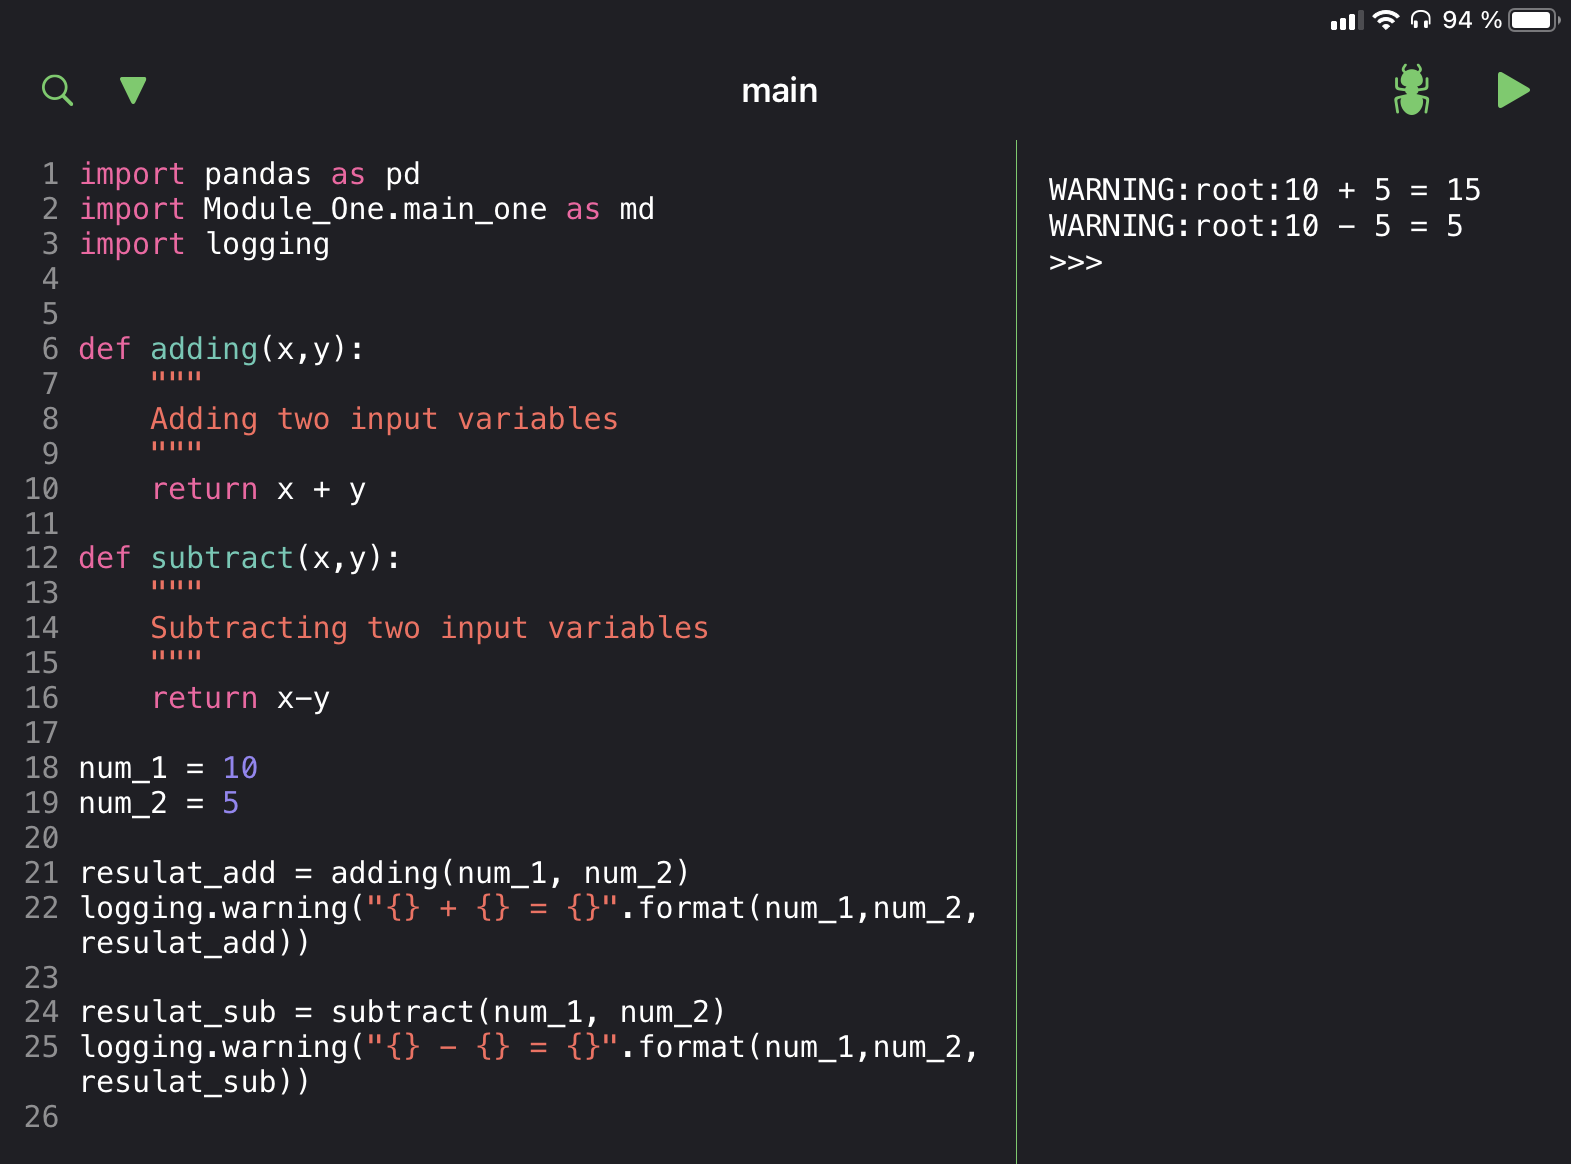
\includegraphics[scale = 0.5]{attachment/chapter_4/Scc025}
\end{figure}

\begin{lstlisting}[style=python]
	import pandas as pd
	import Module_One.main_one as md
	import logging
	
	
	def adding(x,y):
	"""
	Adding two input variables
	"""
	return x + y 
	
	def subtract(x,y):
	"""
	Subtracting two input variables
	"""
	return x-y
	
	num_1 = 10
	num_2 = 5
	
	resulat_add = adding(num_1, num_2)
	logging.warning("{} + {} = {}".format(num_1,num_2, resulat_add))
	
	resulat_sub = subtract(num_1, num_2)
	logging.warning("{} - {} = {}".format(num_1,num_2, resulat_sub))
\end{lstlisting}

Die Konfiguration werden in der Methode \textit{basicConfig()} getroffen. Um anzugeben, ab wann ein Log-Statement ausgegeben wird.
\begin{lstlisting}[style=python]
	%...
	logging.basicConfig(level=logging.INFO)
	%...
\end{lstlisting}
Das Level wird mit einem Integer-Wert bestimmt. Jedes Level lässt sich als Konstante ausgeben.

\begin{figure}[H]
	\centering
	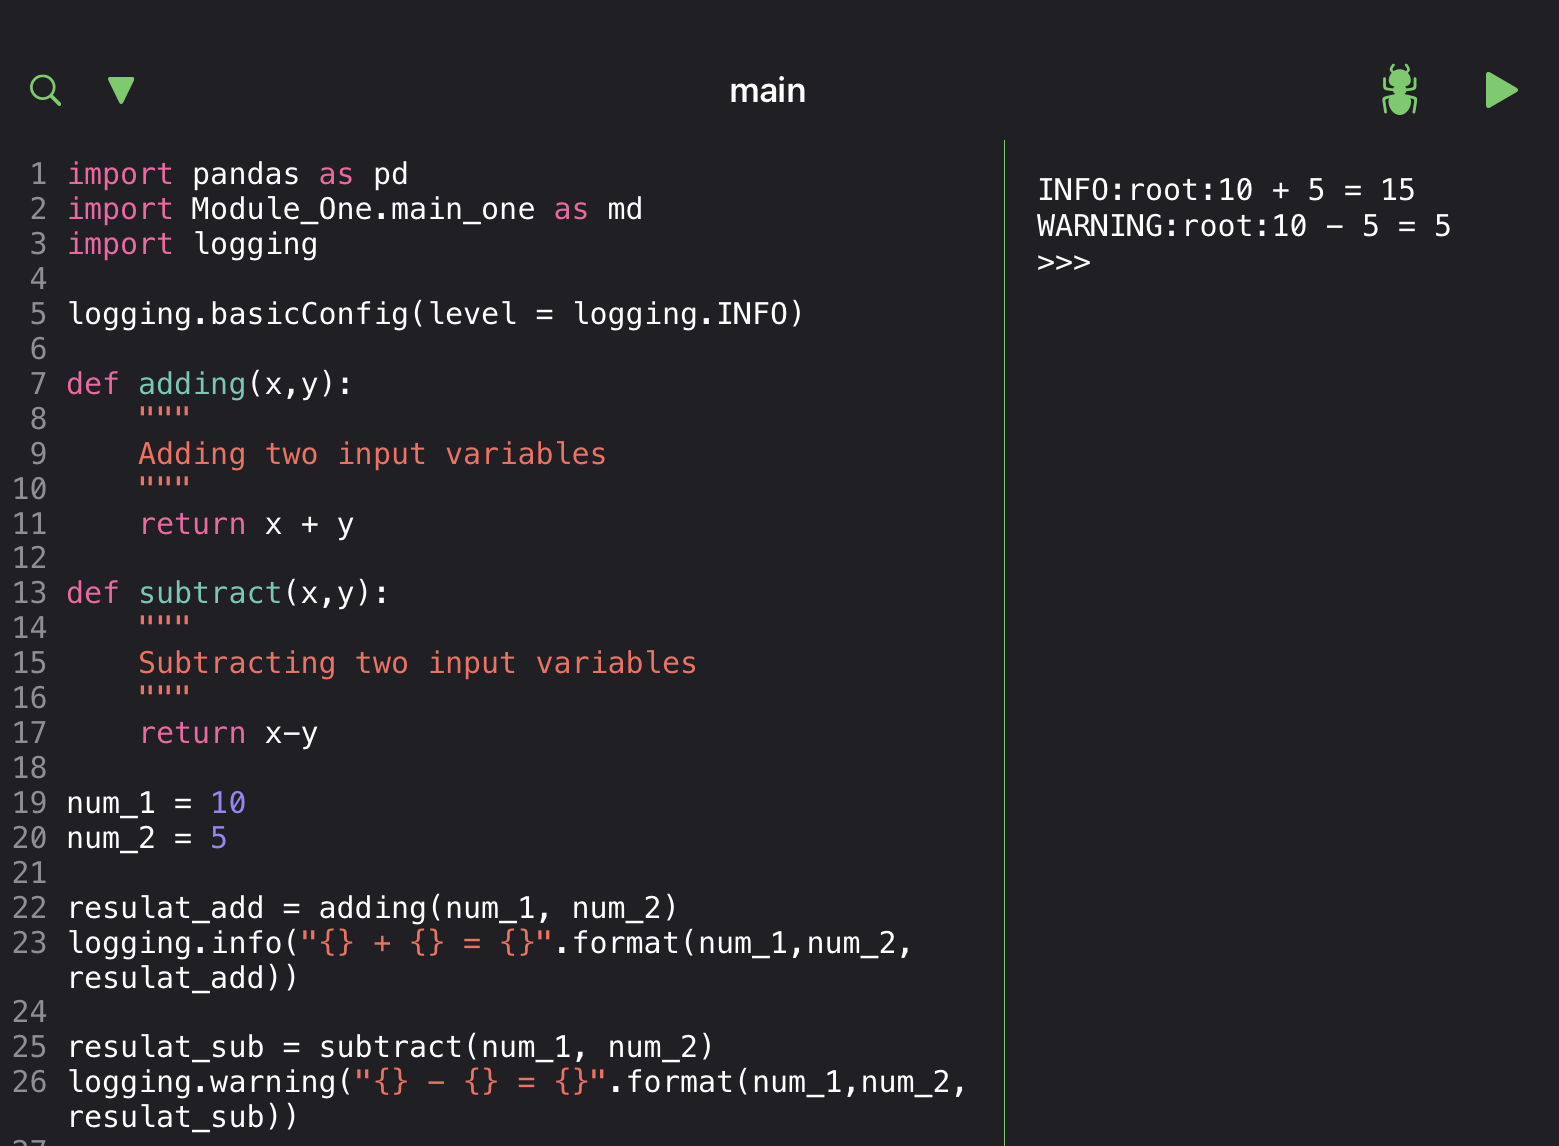
\includegraphics[scale = 0.5]{attachment/chapter_4/Scc026}
\end{figure}

\subsection{Logging to simple file}
Über die \textit{.basicConfig()} Methode kann spezifiziert werden, wo die Log-Statements gespeichert werden.

\begin{lstlisting}[style=python]
	%...
	logging.basicConfig(filename = "log_file.log", level=logging.INFO)
	%...
\end{lstlisting}

\begin{figure}[H]
	\centering
	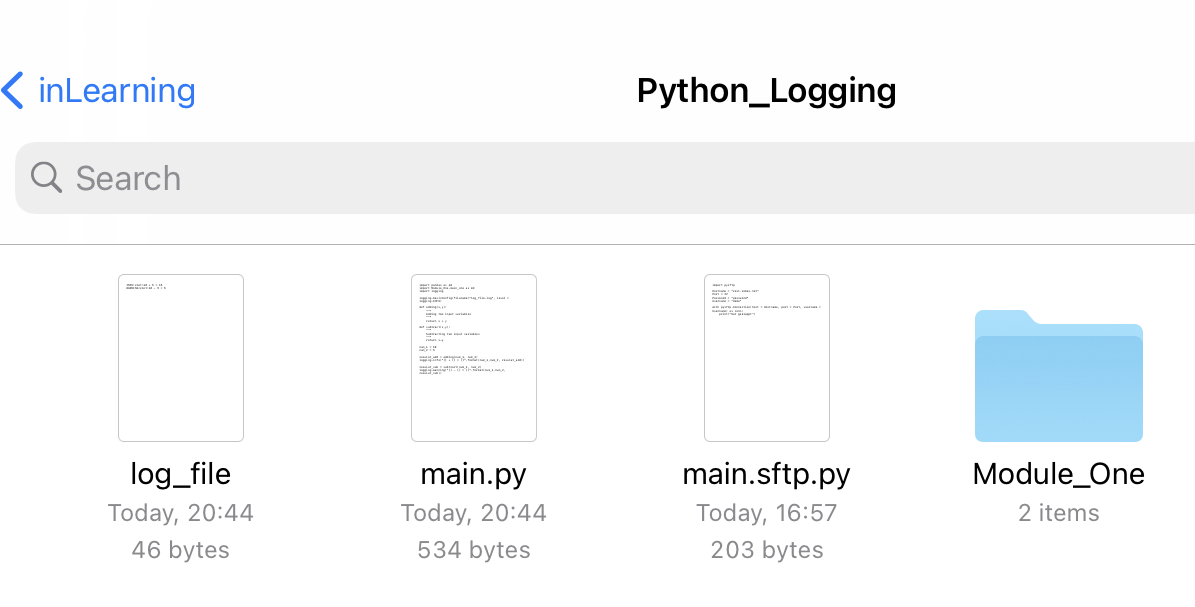
\includegraphics[scale = 0.5]{attachment/chapter_4/Scc027}
\end{figure}
Die Log-Statements werden in der angegeben Datei gespeichert und nicht mehr in der Konsole ausgegeben. In der Grundeinstellung, werden die Logs angefügt, sodass die Logs bei jedem Durchlauf angefügt werden.

\begin{figure}[H]
	\centering
	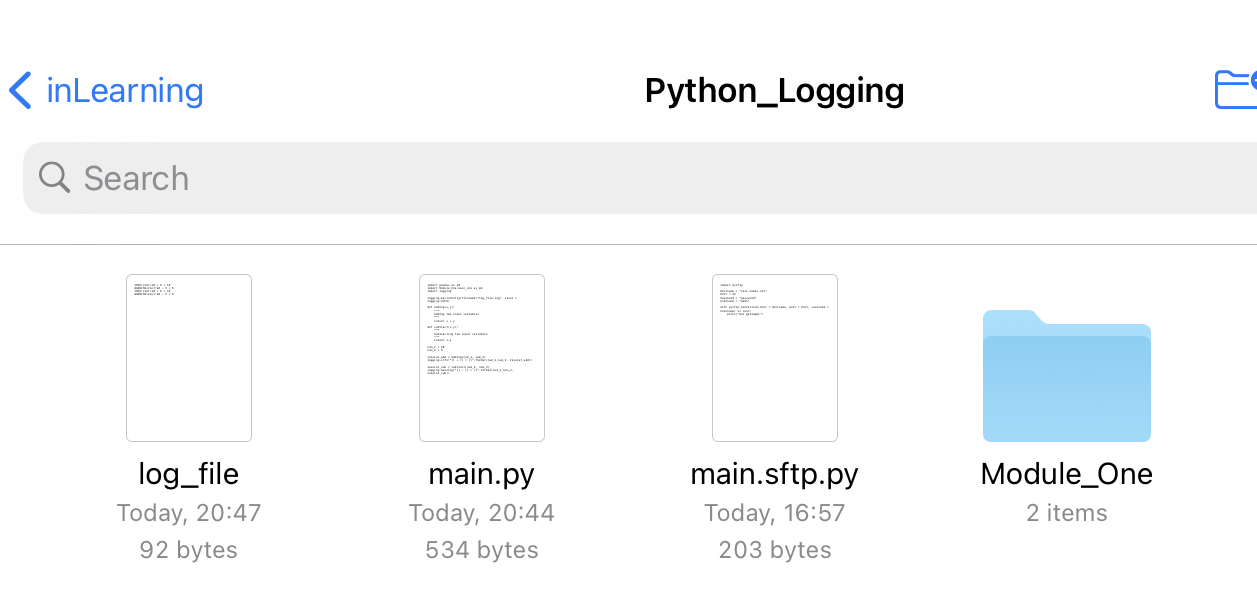
\includegraphics[scale = 0.5]{attachment/chapter_4/Scc028}
\end{figure}

\subsection{basicConfig - Formating}
Unter \href{https://docs.python.org/3/library/logging.html}{Log-Records Attributes} werden die möglichen Attribute für die Formatierung der Log-Statements dargestellt. Die Methode \textit{basis.Config()} bietet unter dem Parameter \textit{format} an, die Ausgaben zentral zu bestimmen. \\

Mit den Variablen 
\begin{itemize}
	\item $\%$(asctime)s
	\item $\%$(levelname)s
	\item $\%$(message)s
\end{itemize}
wird erzeugt: 

\begin{figure}[H]
	\centering
	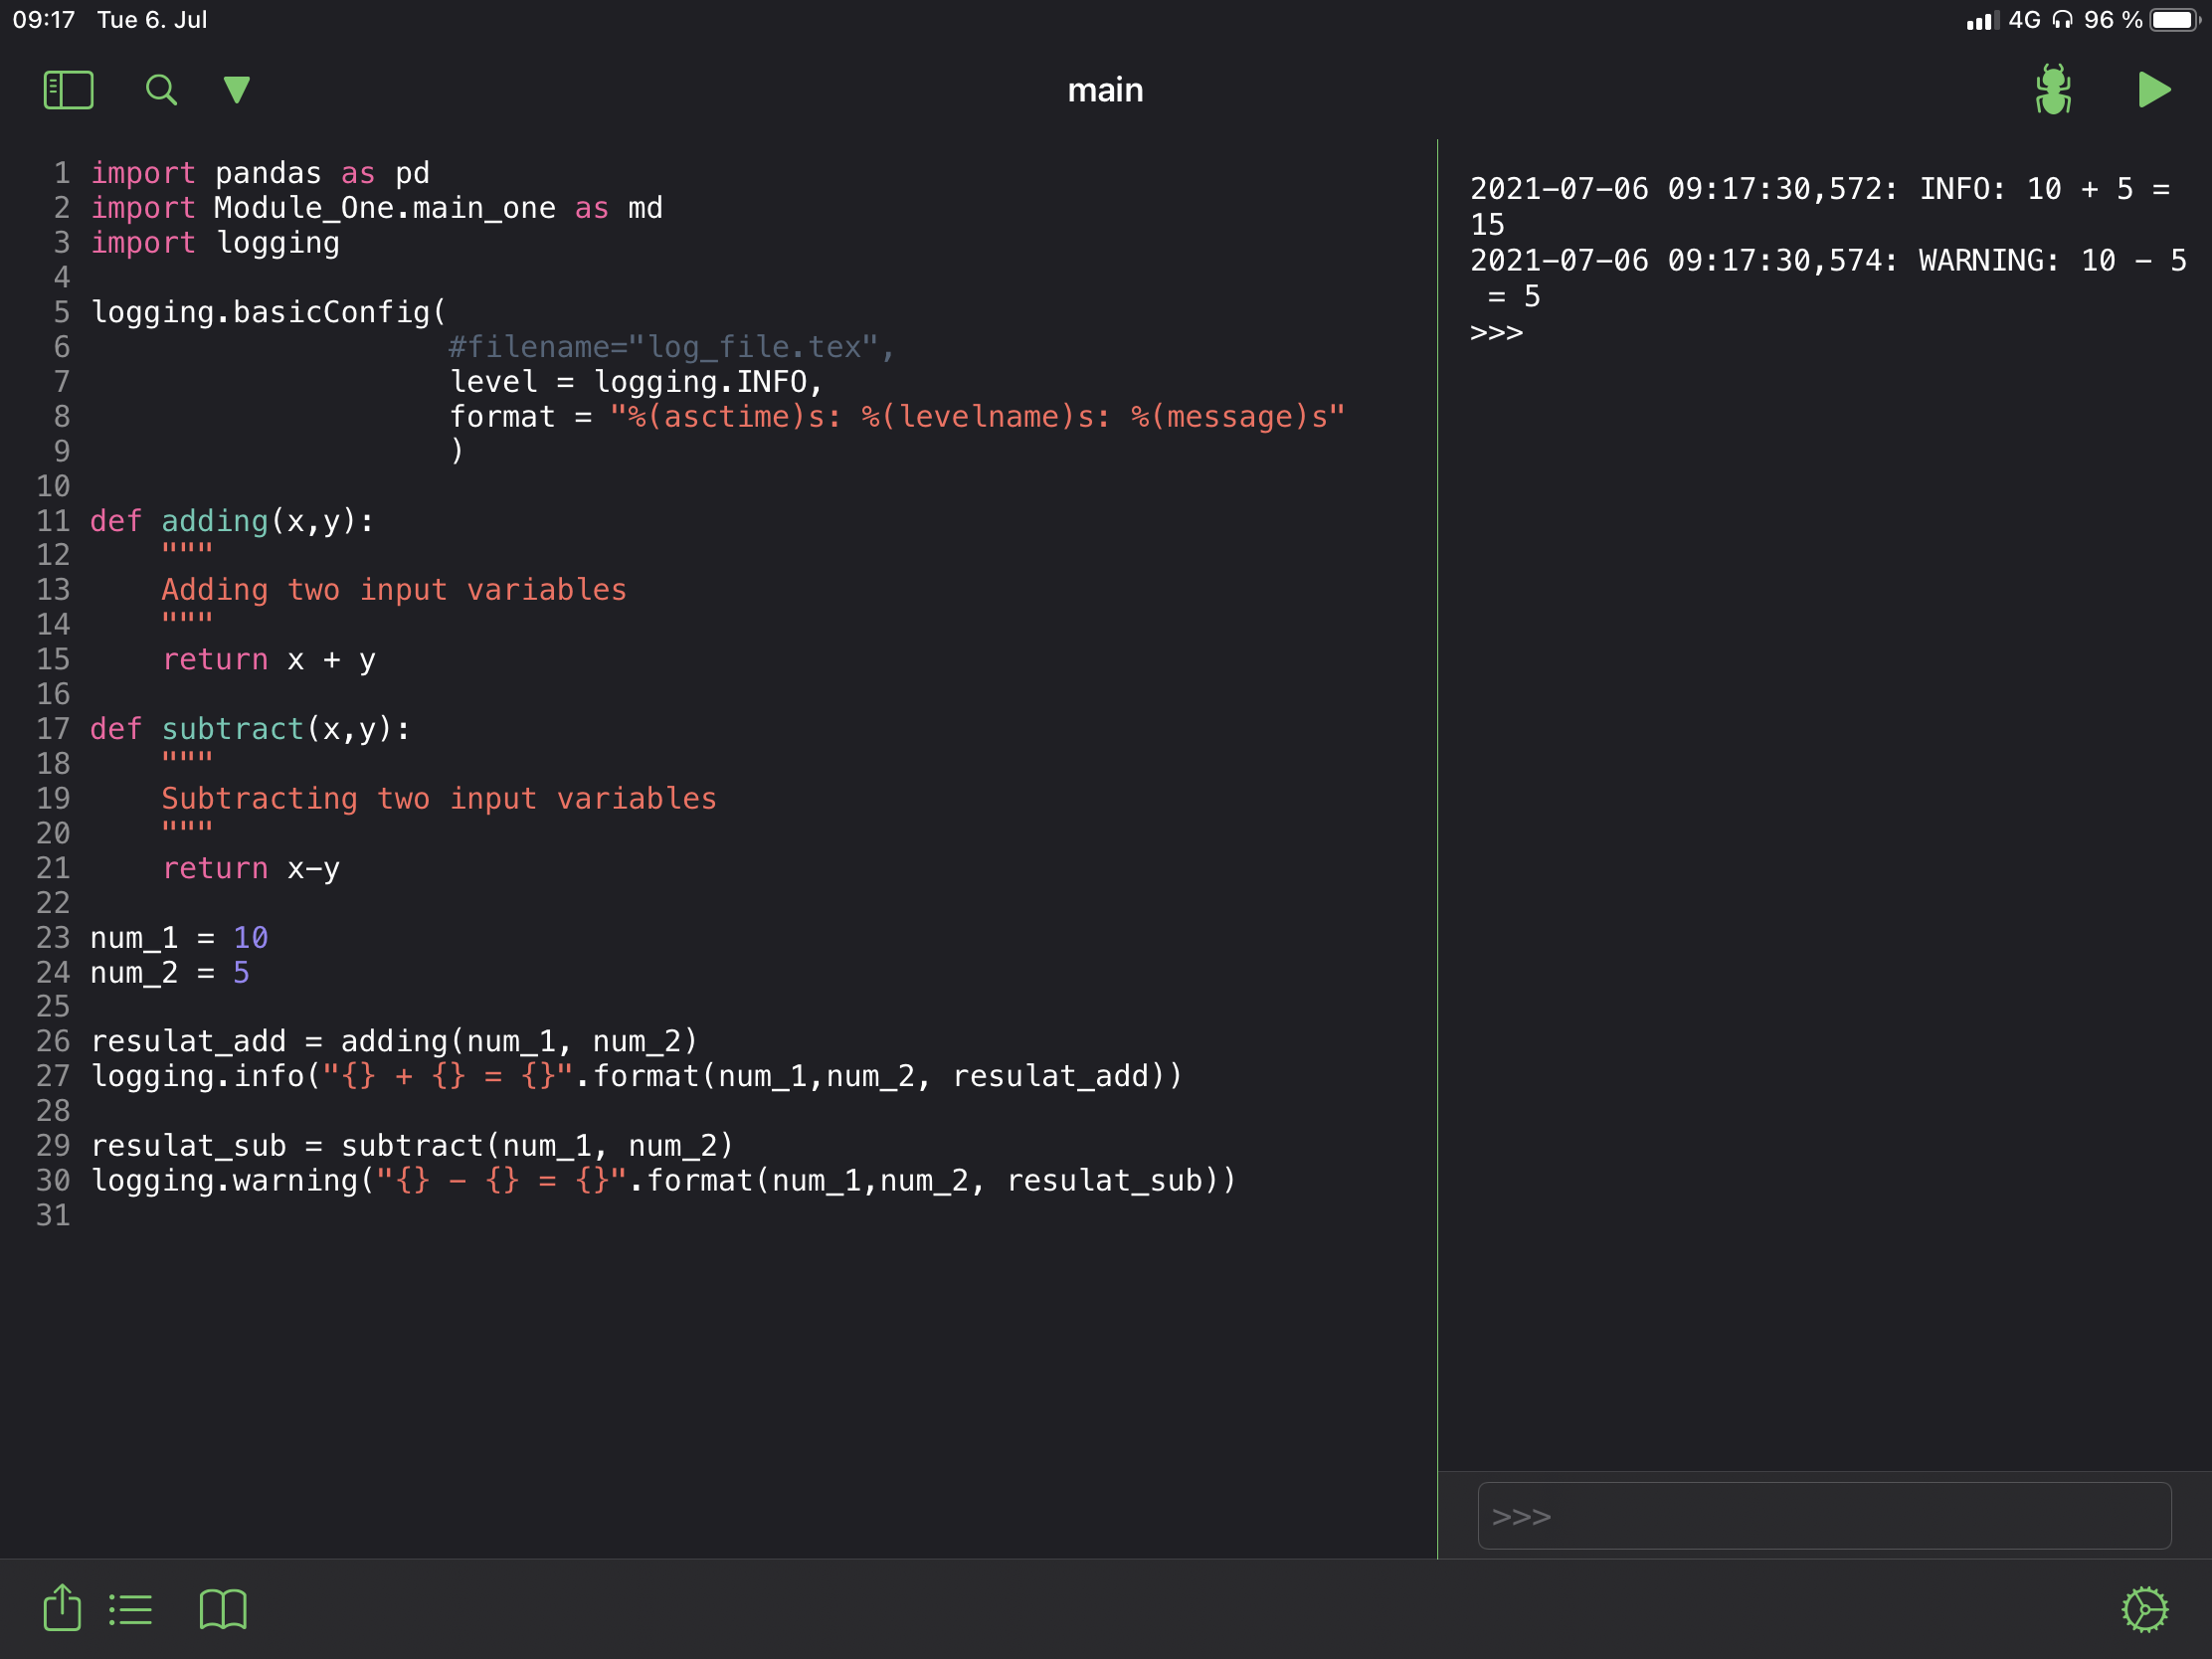
\includegraphics[scale = 0.5]{attachment/chapter_4/Scc029}
\end{figure}

Bei größeren Applikationen werden meist mehrere Module geladen und verarbeitet. 
In den vorherigen Abschnitt wurde sich mit \textit{basicConf()} auf die Grundeinstellung bezogen. Dabei wird diese Funktion nur einmal aufgerufen und ausgelesen, jedes weitere aufrufen wird ignoriert.\\

Dies wird am Beispiel mit zwei Modulen deutlich. In \textit{main.py} mit dem Untermodule \textit{main$\_$one.py}. In \textit{main$\_$one.py} wird die Basis-Formatierung mit :: zwischen jedem Befehl getrennt.  

\begin{figure}[H]
	\centering
	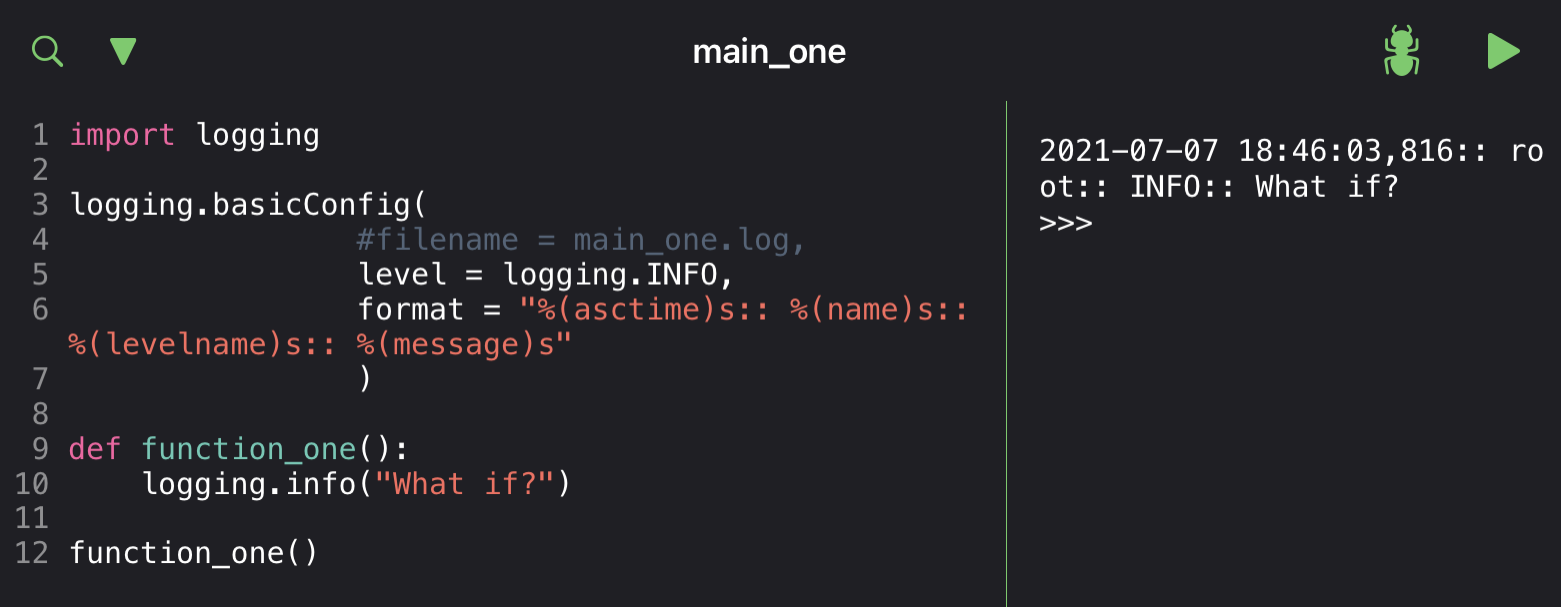
\includegraphics[scale = 0.5]{attachment/chapter_4/Scc030}
\end{figure}

In \textit{main.py} nur mit : $"$.$"$

\begin{figure}[H]
	\centering
	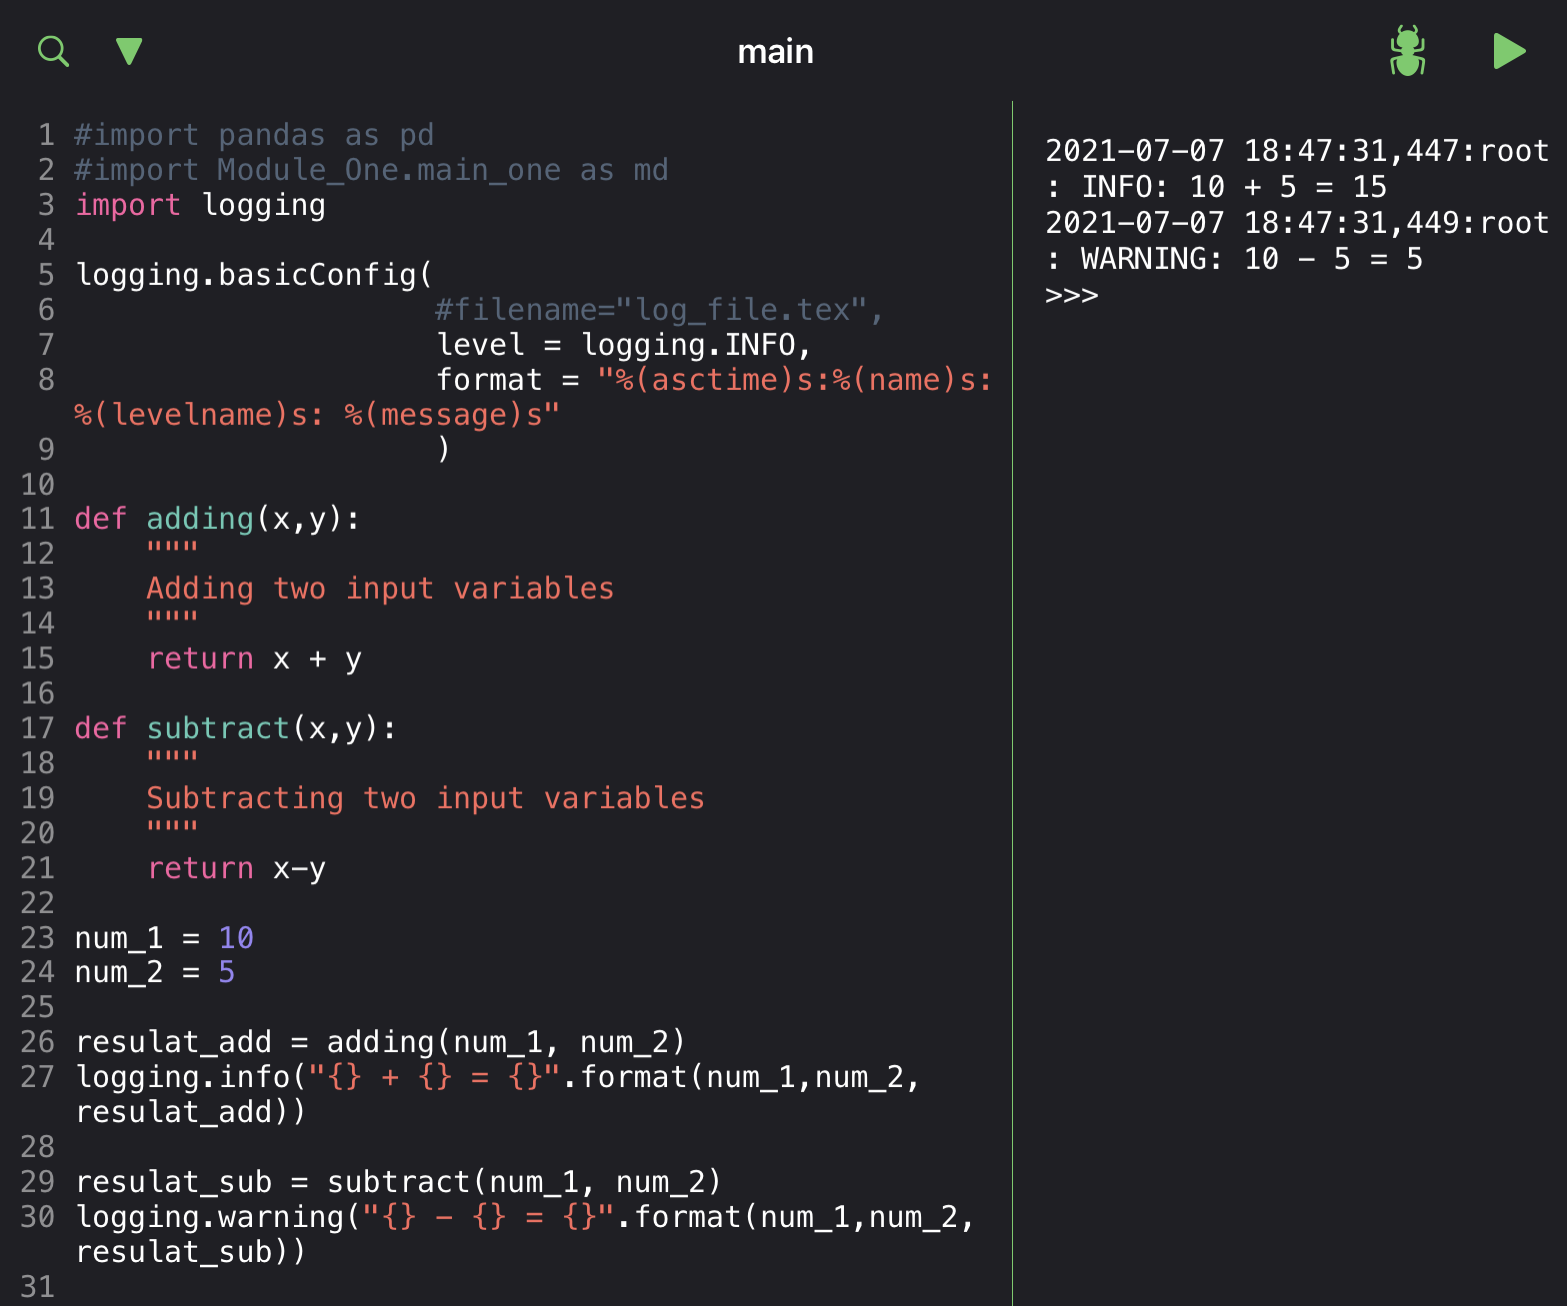
\includegraphics[scale = 0.5]{attachment/chapter_4/Scc031}
\end{figure}
Dabei wurde das Untermodule auskommentiert.\\

Wird das Untermodule zu erstgeladen, so kommt es dazu, was oben beschrieben wurde, die Konfigurationen werden zu erst festgelegt und eine weitere Ansprechung funktioniert nicht.

\begin{figure}[H]
	\centering
	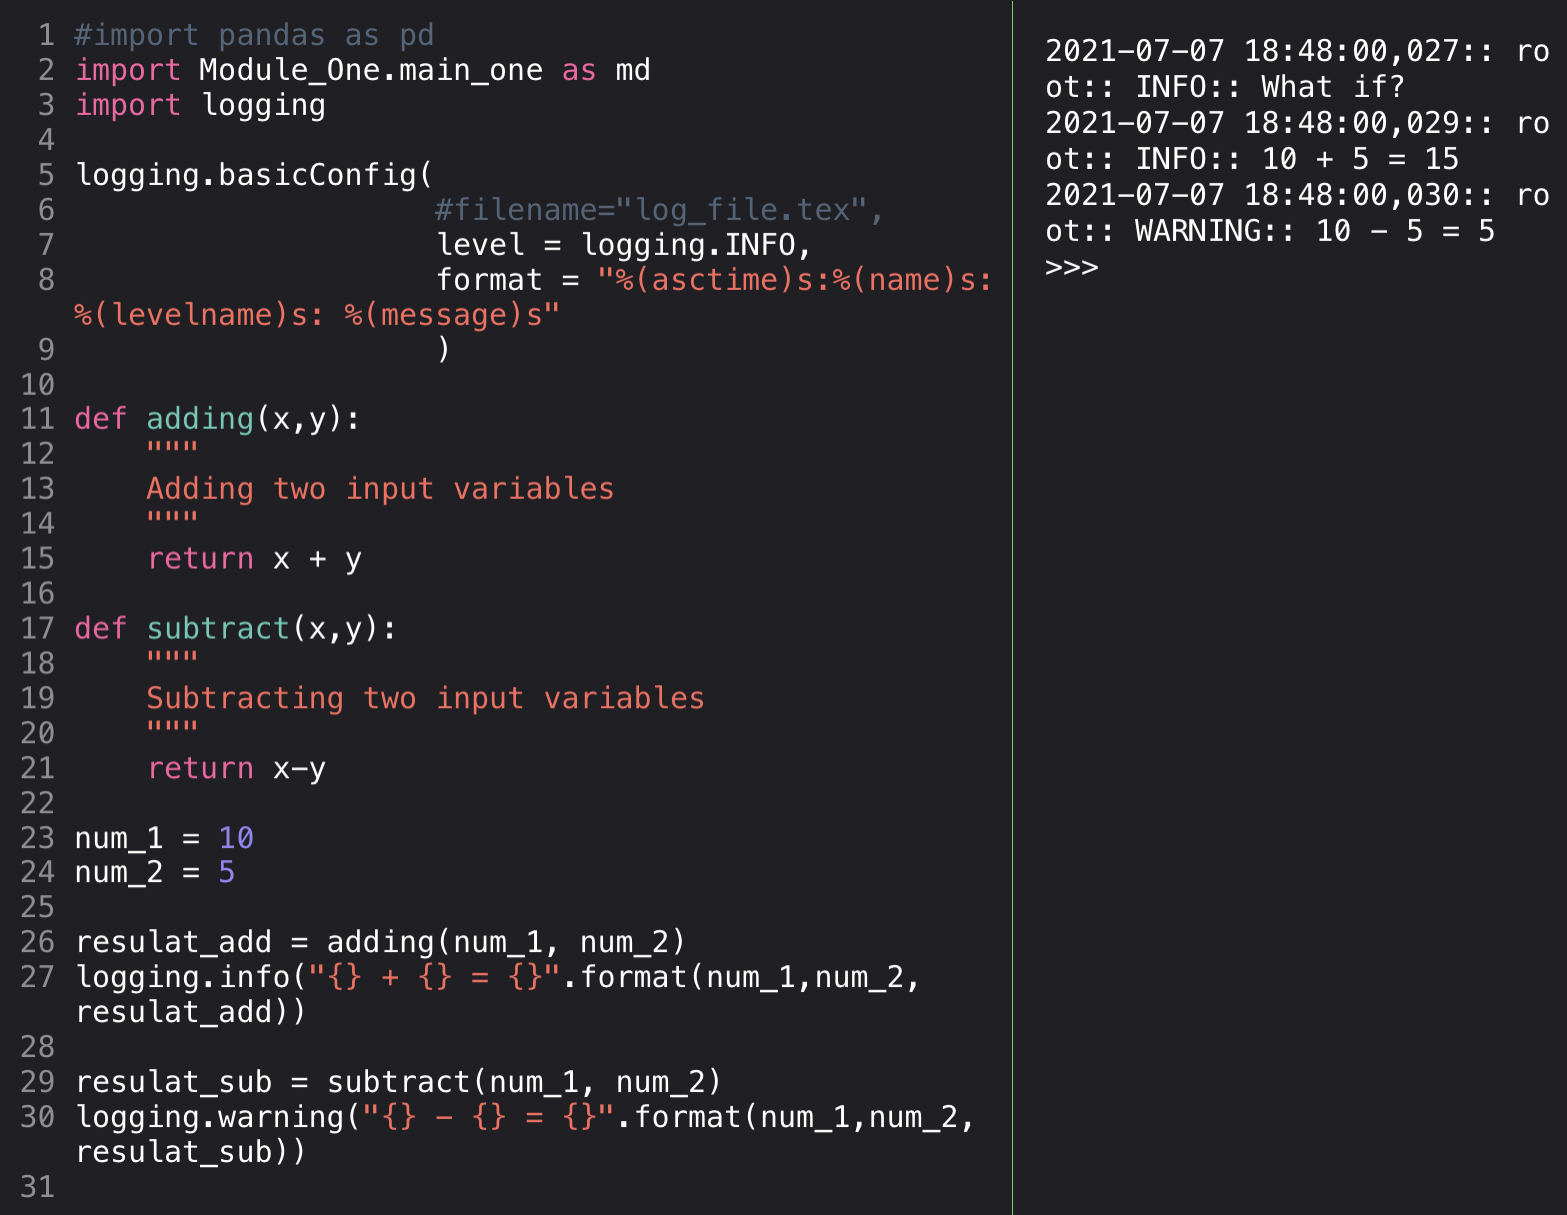
\includegraphics[scale = 0.5]{attachment/chapter_4/Scc032}
\end{figure}

In beiden Fällen bleibt das Verzeichnis \textit{root}, weil das Skript aus \textit{main.py} gestartet wird.

\subsection{Logger, Handler, Formatter}
Um die Komplexität der verschiedenen Module zu bewältigen, wir ein \textit{Logger} erstellt, welcher die verschiedenen Konfigurationen aufgreift. Dieser wird mit \textit{logging.getlogger()} erstellt. 

\begin{itemize}
	\item Der Befehl 
	\begin{lstlisting}[style=python]
		logger = logging.getLogger(__name__)
	\end{lstlisting} führt dazu, dass der Module-Name ausgelesen wird.
	\item Das Level wird über 
	\begin{lstlisting}[style=python]
		logger.setLever(logging.DEBUG)
	\end{lstlisting} 
	\item 	
\end{itemize}

%\begin{figure}[H]
%\centering
%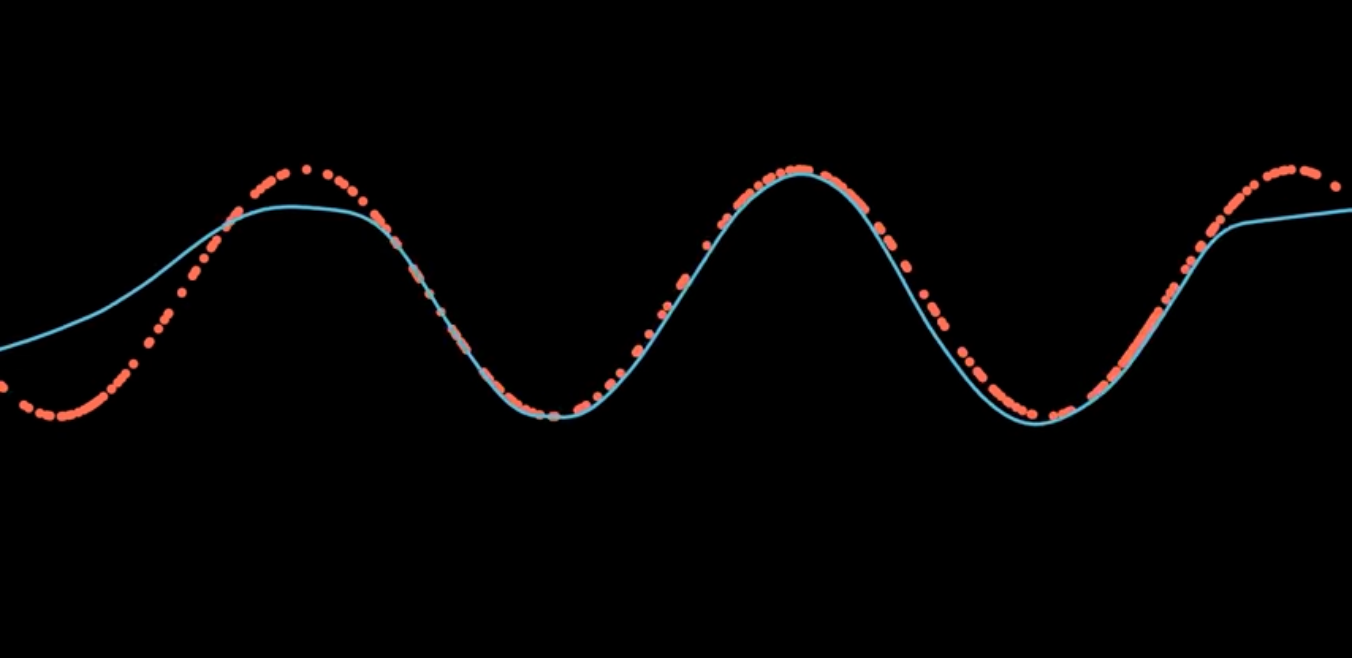
\includegraphics[scale = 0.5]{attachment/chapter_4/Scc033}
%\end{figure}
\section{Documentation}
\subsection{Type Hint}

Um eine genauere Beschreibung von Funktionen und Klassen in Python zu erhalten, bieten sich Type Hints an. Diese geben an, was eine Variable an Input erwartet oder eine Funktion ausgibt. \\
Die Beschreibung ändert jedoch nicht die dynamische Natur von Python. Diese Typ Beschreibungen geben nur ein "Hint" an. Beispiel:
-
\href{https://youtu.be/yScuF1UgGU0}{Link}
Ohne Type Hint
\begin{lstlisting}[style=python]
	# Bevor
	def function(text,key):
	result = ""
	for char in text:
	c = ord(char)
	enc_char = chr(c+key)
	result += enc_char
	return result
\end{lstlisting}
Mit
\begin{lstlisting}[style=python]
	def function(text: str, key: int) -> str:
	result = ""
	for char in text:
	c: str = ord(char)
	enc_char = chr(c+key)
	result += enc_char
	return result
	
	print(function("Franziska, Hase fürs Leben", 2))
	print(function(function("Franziska, Hase fürs Leben", 2),-2))
\end{lstlisting}
\subsection{Docstrings}
Beispiel
\begin{lstlisting}[style=python]
	def string_reverse(str1):
	'''
	Returns the reversed String.
	
	Parameters:
	str1 (str):The string which is to be reversed.
	
	Returns:
	reverse(str1):The string which gets reversed.   
	'''
	
	reverse_str1 = ''
	i = len(str1)
	while i > 0:
	reverse_str1 += str1[i - 1]
	i = i- 1
	return reverse_str1
\end{lstlisting}

Dabei können sich mehrer Style unterscheiden. Im folgenden wird Numpy-Style aufgezeigt
\begin{lstlisting}[style=python]
	class Vehicles(object):
	'''
	The Vehicles object contains lots of vehicles
	
	Parameters
	----------
	arg : str
	The arg is used for ...
	*args
	The variable arguments are used for ...
	**kwargs
	The keyword arguments are used for ...
	
	Attributes
	----------
	arg : str
	This is where we store arg,
	'''
\end{lstlisting}

\subsection{Definition of Variables}
Kernfragen: Wie kann zwischen datentragenden Variablen, Hilfs-datentragenden, Objektvariablen oder anderweiligen Variablen unterschieden werden?

Sammelsurium
Die Frage die sich stellt, ist, ob die Metainformation am Anfang oder am Ende der Variablen stehen soll. Ich vermute, es ist leichter zufolgen, wenn gleich zum Anfang klar ist, um welche Kategorie es sich handelt. Der Nachteil ist, sobald man weiß, welche Variable wo steht, entsteht eine gewisse Redundanz. 

Erster Vorschlag:
\begin{itemize}
	\item Data$\_$Storage$\_$Inhalt
	\item Data$\_$Help$\_$Inhalt
\end{itemize}

Es sollte ein Abkürzungsverzeichnis am Anfang für die Legende der Variablen existieren. 
Zum Beispiel sollte anstatt DataStore$\_$Inhalt DS$\_$Inhalt stehen.
\begin{comment}
\begin{comment}
	
	\section{Single Items}
	\begin{description}
		\item[Packages] How to write packages  \href{https://uoftcoders.github.io/studyGroup/lessons/python/packages/lesson/}{Link}, 	\href{https://the-hitchhikers-guide-to-packaging.readthedocs.io/en/latest/quickstart.html}{Link}
		\item[Search in Subset] \href{https://stackoverflow.com/questions/8711596/python-3-s-for-s-in-subsetss-and-yield/8712073}{Link}
		\item[Optimize Pandas for speed] \href{https://engineering.upside.com/a-beginners-guide-to-optimizing-pandas-code-for-speed-c09ef2c6a4d6}{Link}
		\href{https://www.youtube.com/watch?v=nxWginnBklU}{Link}
	\end{description}			
\end{comment}	
	Inhalt...
\end{comment}
